\documentclass[11pt,a4paper,notitlepage]{article}
\usepackage[margin=1in]{geometry}
\bibliographystyle{plain}
\usepackage[utf8]{inputenc}

%\pdfminorversion=6

\usepackage[colorlinks = true,
            linkcolor = black,
            urlcolor  = black,
            citecolor = black,
            anchorcolor = black]{hyperref}
\usepackage{url}\urlstyle{same}

\usepackage[parfill]{parskip}
\setlength{\parskip}{\baselineskip}

\usepackage[compact]{titlesec}
\titlespacing{\section}{0pt}{*0}{*0}
\titlespacing{\subsection}{0pt}{*0}{*0}

\usepackage[backend=biber]{biblatex}
\addbibresource{sources.bib}
\usepackage[nottoc,notlot,notlof]{tocbibind} %TODO: Include References in Table of contents

\usepackage{booktabs}

\usepackage{amsmath}
% Removes most of whitespace above and below equations.
\newcommand{\zerodisplayskips}{%
  \setlength{\abovedisplayskip}{-10pt}% Default: 12pt plus 3pt minus 9pt
  \setlength{\belowdisplayskip}{0pt}% Default: 0pt plus 3pt
  \setlength{\abovedisplayshortskip}{-10pt}% Default: 12pt plus 3pt minus 9pt
  \setlength{\belowdisplayshortskip}{0pt}% Default: 7pt plus 3pt minus 4pt
}
\appto{\normalsize}{\zerodisplayskips}
\appto{\small}{\zerodisplayskips}
\appto{\footnotesize}{\zerodisplayskips}

\usepackage{graphicx}
\usepackage{float}
\usepackage{wrapfig}

% Rename "Figure" in figure captions to "Screenshot"
\usepackage[labelformat=default,font=it,labelfont=bf]{caption}
\captionsetup[figure]{name=Screenshot}

\usepackage{listings}
\usepackage{color}

% <define code listing style>
\definecolor{codegreen}{rgb}{0,0.6,0}
\definecolor{codegray}{rgb}{0.5,0.5,0.5}
\definecolor{codepurple}{rgb}{0.58,0,0.82}
\definecolor{backcolour}{rgb}{0.95,0.95,0.92}
\definecolor{blue}{rgb}{0.0, 0.0, 1.0}
\definecolor{anti-flashwhite}{rgb}{0.95, 0.95, 0.96}
\definecolor{amaranth}{rgb}{0.9, 0.17, 0.31}

\lstdefinestyle{mystyle}{
    backgroundcolor=\color{anti-flashwhite},   
    commentstyle=\color{codegreen},
    keywordsprefix={@},
    keywordstyle=\color{blue},
    numberstyle=\tiny\color{codegray},
    stringstyle=\color{amaranth},
    basicstyle=\ttfamily,
    breakatwhitespace=false,         
    breaklines=true,                 
    captionpos=b,                    
    keepspaces=true,                 
    numbers=left,                    
    numbersep=5pt,                  
    showspaces=false,                
    showstringspaces=false,
    showtabs=false,                  
    tabsize=2,
}

\lstset{style=mystyle}
% </define code listing style>

\usepackage[table]{xcolor}

\usepackage{array}

% Allow additional line-breaking with tolerable white space per line increased by
% 1em. Helps with "Overful \hbox" error in bibliography.
\emergencystretch=1em

\usepackage[T1]{fontenc}
\newcommand\bslash{\char`\\}

\begin{document}
\begin{centering}
\centering
    
    \rule{\textwidth}{1.6pt}\vspace*{-\baselineskip}\vspace*{2pt}
    \rule{\textwidth}{0.4pt}\\[\baselineskip]
    {\LARGE \textbf{Coinz: Implementation Report} \\[0.5\baselineskip] Sebastian Müksch} \\[1\baselineskip]
    {2018/12/02}
    \rule{\textwidth}{0.4pt}\vspace*{-\baselineskip}\vspace{3.2pt}
    \rule{\textwidth}{1.6pt}\\[\baselineskip]
\end{centering}

\tableofcontents
\newpage

\section{Implementation Description}

\subsection{Handling the GeoJSON Map}

    Each new GeoJSON map, i.e. coin map, goes through the same 3 steps within the application:

        \begin{enumerate}
            \item Downloading the GeoJSON file
            \item Parsing the GeoJSON file
            \item Storing the parsed data in a local SQL database
        \end{enumerate}

    To keep the UI from being blocked, Android requires that tasks like accessing remote content be one in a separate thread. Therefore, the GeoJSON file is downloaded through an AsyncTask that runs in the background, fetches the file and returns it as a string to be process further. \cite{async-task}

    Parsing the GeoJSON into actual objects the rest of the code can work with happens partially using Mapbox's FeatureCollection class \cite{feature-collection} and partially using Java's JSONObject class. \cite{json-object} The former is used to parse all the features, i.e. coins, within the GeoJSON map into actual coins as it provides a simple way to run through all them. The latter is used to extract information about the GOLD exchange rates for the day from the GeoJSON file.

    Lastly, once the data is parsed into objects, the Room Persistence Library \cite{room} is used to store the generated objects within a local SQL library. The actual details are hidden by the Room library, as it is an abstraction layer to SQLite, but the way it is implemented is via an INSERT query that is requested from Room for both coin data and GOLD exchange rates.

\subsection{Persistent Local Storage}

    With exception to the download date of the currently displayed map, which is stored as a key-value pair in the SharedPreferences, the bulk of the locally stored data is kept within an SQL database managed by the Room Persistence Library. \cite{room}

    The rationale behind using Room to manage the local data is three-fold:

        \begin{enumerate}
            \item The data necessary for the application to run is highly structured, i.e. we know ahead of time that each coin will have a certain number of attributes attached to it, making it a good candidate for an SQL database.
            \item Storing the coin data in a parsed manner, especially inside an SQL database, saves time accessing the data as it will only have to be parsed when it is downloaded and is then readily available through queries which directly return instances of a class.
            \item The Room Persistence Library as an abstraction layer to SQLite offers a tremendous pool of utilities simplifying the procedure of having an SQL database connected to the app enormously. Room for instance provides compile-time checked SQL queries as well as the option to set observers on data in such a way that we can implement a general notification throughout the app should a coin be for instance collected. This makes keeping the UI up-to-date essentially trivial.
        \end{enumerate}

    On top of all that, the Room Persistence Library interacts well with the concept of ViewModels, which offer us a way of keeping data apart from UI in a lifecycle conscious way. \cite{view-models}

\subsubsection{Entities}

    Coins, which in effect work as markers as well since they always have a position attached to them, are implemented as so call Entities \cite{room-entities}. This means that each coin will be stored as a row in the local SQL database. The same holds for each GOLD exchange rate, which are also implemented as entities and stored as rows in their own table within the local SQL database.

\subsubsection{Repositories}

    Since we have already established that we are only going to parse a coin map once, at the time it is downloaded, then access the local SQL database to query the data within it, it is reasonable to suggest to only download a coin map when the old one expired and not every time the app starts up again. However, it would be quite tedious to have the logic to take care of this everywhere we need to access the coin data. I have therefore made use of a so-called Repository, which is essentially an abstraction layer that abstracts the logic of whether to download a new map, i.e. access the network, or use local data. Repositories are also part of the recommended app architecture. \cite{app-arch-guide}

    The way this works in the background is that the last date a map has been downloaded is kept within the SharedPreferences and every time an access to the local SQL database is requested, this last download date will be checked against the current date. Since coin maps expire with every new day, should last download and current date be different, a download through an asynchronous task is started, otherwise the data request is forwarded to the Room Persistence Library which handles the local database. There is a repository each for both coin entities and GOLD exchange rate entities.

\subsubsection{View Models}

    One last layer of abstraction that is added atop the repositories is view models. \cite{view-models} The reasoning behind adding another layer to the local data is that when data is kept within the UI controller and it gets destroyed and re-created, any data stored within them will be destroyed. To keep that from happening, any data that is needed by the UI will be kept separate from the UI controllers in view models that manage them.

\subsection{User-to-Coin Distance Detection}

    The distance calculation between each coin and the user is deceptively simple. Within the fragment that manages the map, the user's position is kept constantly updated. When the user presses on a coin marker, the marker will have a latitude and a longitude. These values are both taken and using the built-in distance calculation functionality from Mapbox's LatLng class \cite{lat-lng}, the distance is computed.

\subsection{Coin Collection}

    Since in this implementation of the Coinz app, coins are not collected automatically, the user will be prompted with a collection dialog each time they click on the marker of a coin they would like to collect. As they cannot collect coins further than 25 meters from them by specification, the user-to-coin distance calculated above is passed to the dialog fragment that implements the coin collection dialog and if the user is too far away from a coin, the collection button is blurred out, i.e. disabled. If the user is close enough, the button becomes active and the user can collect the coin, in which case an internal flag within the SQL database is set for the coin in question, marking it as collected and the markers on the map are redrawn with the collected coin now not shown.

\subsection{Switching Between Interfaces}

    The core interfaces for the player are the map, the Local Wallet and the Central Bank. All of these are implemented via Fragments \cite{fragments} which are all part of the main activity. The user can switch between the map, the Local Wallet and the Central Bank through a navigation drawer on the left. Upon pressing on for instance the Local Wallet when currently being on the map, the active fragment is replaced with the requested fragment, taking the user to the interface they desire.

\subsection{Local Wallet and Banking Coins}

    While currently not functioning, see details below, the feature to bank coins is of the Local Wallet. Within the Local Wallet, all collected coins appear as cards in a list of collected coins. Within each card is a button "Store", which opens a dialog window to bank the coin into the Central Bank. The dialog window shows some key information related to the banking process, namely the effect on the GOLD amount the user currently possesses. This means that each coin has a separate button to be banked individually from all other coins. As a matter of fact, each coin also has a separate "Send" button to send the coin to another user, however, this feature has not been implemented, see details below.

\subsection{Account Management}

    A big part of the Coinz app is being able to log in with an account to access online features such as the Central Bank and send spare change to other users. The account management in the background is implemented using Firebase authentication with email and password.

    To log in to an existing account, a login screen is provided which is implemented in such a way that it is the first screen that appears for the user when they first open up the app after a download. Should the user not already have a Coinz account, a button for them to create one is provided on the login screen which takes them to an account creation screen. There, the user can enter an email address and a password, which are passed to the Firebase authentication in the background and handled on their end.

\section{Not Implemented}

\subsection{Banking Coins}

    Due to a last-minute breakdown of the Firestore related code, see \cite{firestore-issue}, I have had to remove the parts of the app which accessed Firestore to keep the app from crashing. Unfortunately, this implies that the user is not able to bank their collected coins into the Central Bank. However, the UI to do so still exists and when the user attempts to bank a coin it will be removed from the Local Wallet, but the GOLD amount of the user will not increase.

\subsection{Sending Coins}

    Another consequence of the previously mentioned Firestore issue is that I could not implement the feature that would allow the user to send collected coins to other players and also receive spare change sent by others. This feature would have required the use of a Firestore database, which would have inevitably crashed the application for reasons that I did not have the time to analyze, let alone fix before the deadline.

\subsection{Bonus Feature: Spare Change Multipliers}

    In addition to the required features above, one of my bonus features also had to be removed from the submitted version, as it relied on sending spare change. In order to have players actively engage in a Coinz player community, I had envisioned what I refer to as a Spare Change Multiplier. In essence, it is a reward system for corporation in which each player would get a random multiplier for a randomly chosen currency each day which would increase the value of spare change received in that particular currency. However, if spare change cannot be sent between player due to an unresolved Firestore issue, there cannot be a Spare Change Multiplier.

\subsection{Unit and Integration Test Coverage}

    As described in the original plan, I wanted to implement Unit tests and Integration tests for as much of the application as possible. However, due to time being very limited with an approaching deadline, I was not able to implement proper test coverage. There are some Unit tests which have been implemented, but it is far from what I originally planned.

    An additional factor weighing in on this is the fact that I had anticipated how complex it would be to write proper Unit tests for Android app components. A sizable part of my code relies on Android components like application contexts being present. These would have to be mocked for the tests, which turned out to be more complex than originally assumed. Therefore, the test coverage of my application is rather poor compared to what was originally planned.

\subsection{Espresso Test Coverage}

    In my original plan I wanted to have a wide coverage of the application's UI with Espresso tests. However, there were two major issues which kept me from achieving this goal.

    The first issue is related to the very nature of the Coinz game. Many aspects of the game and its current implementation change with environmental factors such as the date. For instance, each day a new coin map is released with always different marker positions, which makes it hard to consistently test for something like marker clicks or the values that should appear when a marker is eventually clicked. The same goes for the Local Wallet, which depends entirely on the already collected coins. I have therefore not been able to find a way to create a mocked environment in which separate parts of the UI can be tested in a consistent way.

    The second issue is related to AndroidStudio and a problem that I had while trying to record Espresso tests. \cite{espresso-issue} While trying to record tests and adding assertions, the tool within AndroidStudio that would normally do so failed to get the UI hierarchy. Without this step, however, no assertions could be added which essentially means that no test is being recorded. At one point, for reasons that I do not know, the test recorded was actually able to capture the UI hierarchy and it let me create a test. However, immediately after the tool broke down again. I was finally able to record some tests when hooking AndroidStudio up to a physical Android device, but this partial fix to the problem came rather late.

\section{Known Issues}

    This is a compilation of issues which have been identified while working on the implementation and testing it but could not be resolved in time for the submission deadline.

\subsection{Freezing with Navigation Drawer}

    One particular issue that surface rather late into the implementation of the application is that if the user selects either the Local Wallet or the Central Bank item in the navigation drawer and then selects the same item another time, the app freezes and eventually gets forced to shut down. The best analysis that I could find as to why this happens is that it is seemingly cause by the way the application replaces fragments upon clicking an item in the navigation drawer.

    When removing the bit of code that replaces the fragment within the fragment container, the application functions without an issue, apart from the fragments not being put into action. However, despite trying to reuse fragment objects and multiple checks whether the current fragment is the same that the fragment container should be filled with, the issue still persists.

\subsection{Refreshing of Location Permissions}

    Another issue that has surfaced when testing the application is that when the user first installs the app and runs it, they will be prompted for the location permissions. If the user accepts right-away, everything seems to work as planned. However, should the user first deny the permission, they will immediately be prompted for it again in if the user then accepts it, the permission dialog will go away but the location will in fact not be updated like it would if the user had accepted the location access of the app from the get-go.

\subsection{Locality of the Local Wallet}

    As described earlier, the local data used by the application is stored within an SQL database managed by the Room Persistence Library. However, as the current implementation stands it is not checked which user is logged into the Coinz at the current moment. Therefore, if user A was to log in, collect some coins and then log out again with user B logging in after them, user B would see the coins collected by user A within their Local Wallet.

    Additionally, given the scenario above, if user A was to install the app on a different device and log into their account, they would see no coins within their Local Wallet, especially not the coins they collected on the other device.

    The reason for this is that the Local Wallet really is implemented \emph{locally}, i.e. it is not synchronized with any online database at the current iteration of the app.  This tracks back partly to the Firestore issue. \cite{firestore-issue}

\subsection{Going Back on Login Screen}

    While on the login screen, if the user presses the back button on their phone, the login screen will appear to be refreshed and the user will be prompted for location permission access, if they have not given it to the application yet. The same behavior seems the occur when going from the login screen to the account creation screen and then pressing the back button, taking the user back to the login screen and showing the permission request.

    My best analysis of the situation so far is that the map fragment is the default fragment within MainActivity. When the user starts up the application, the MainActivity is launched and immediately passes over to the login screen, should it find that the user is not logged in. When the user then presses the back button, the app goes briefly back to the MainActivity, where it for reasons I could not analyse yet, tries to access the map fragment which will then trigger a permission request. This appears to be happening quickly enough such that it is triggered within the short amount of time that the app takes to load the login screen again.

    A potential solution may be to make the login activity the launch activity, however, this has cause issues with starting the app in the past and has hence been avoided in the current implementation.

\section{Additionally Implemented}

\subsection{Fragments}

    In the original design plan for Coinz I had detailed the use of various activities to handle different parts of the application. In particular, I had planned to implement the following features as activities:

    \begin{itemize}
        \item Map
        \item Local wallet
        \item Central Bank
        \item Sending spare change
    \end{itemize}

    Upon reading up on Fragments \cite{fragments} it became clear that a more appropriate implementation of the above features would involve fragments for each of them, rather than separate activities. 

    The decision of using fragments for the features listed above is that they give bigger freedom in designing the UI of the game. Currently and just as planned in the design document, the user switches between map, Local Wallet and Central Bank through a navigation drawer, a behavior which in theory could be implemented using activities as well. However, activities are very rigid in terms of restructuring the UI. For example, should Coinz be adapted for larger screen sizes, for instance a tablet, then fragments would allow a simple redesign of the UI, for instance displaying the map on one half of the screen and the Local Wallet and Central Bank on the other. This is not possible if map, Local Wallet and Central Bank are implemented as activities.

\subsection{Log In and Account Creation}

    Not detailed in the original design document, yet essential to the online aspect and player interaction in Coinz is the ability to create a player account and to log into it when starting the app. Therefore, an activity to log into an account managed by the Firebase service has been added. The login activity will create a login screen which is the entry point for the application when the user first opens the application. In case the user has already logged in in the past, the application will go straight to the map to allow the user to play the game.

    Additionally, the login screen provides a button formatted as a link you would typically see on a webpage, which will take the user to the account creation screen on which they can sign up to Coinz with an email address and a password, should they not already possess an account.

\subsection{Marker Multipliers - A Minor Change}

    In the original plan I had designed the marker multipliers, which from here on out I will refer to as marker color multipliers, to give a multiplier for a coin value when collected with a particular color during a particular time of day depending on the hue of the marker color. All this has been implemented as planned, with the minor adjustment that the multiplier is now the same for each marker color regardless the hue to make the game mechanic fairer and not favor one currency over the others.

\subsection{Bonus Feature: Symbol Multipliers}

    Recall that one of the originally planned bonus features, namely the spare change multipliers, could not be implemented due to Firestore not working \cite{firestore-issue}. To mitigate the negative effects of this, I have implemented a different bonus feature which is similar to the first bonus feature of marker color multipliers.

    The way the symbol multipliers work is quite simple: each marker has a symbol with a digit from 0 to 9 on them. If the last digit of the current day of month, e.g. 7 for the 17th., 2 for the 2nd, is equal to the symbol on the marker of the coin, then the coin value gets multiplied by a multiplier upon collecting the coin. This bonus feature is compatible with the marker color multipliers as all multipliers will just stack on top of each other.

    The added benefit of this bonus feature is that the players are incentivized to not only play the game regularly throughout the day to get multipliers for coins with particular colors at particular times of the day, but also to play it regularly throughout the month as each day a different kind of marker will give favorable advantages.

\section{Reflection}

    Before moving on to the application showcase to demonstrate what of my original plan has actually been implemented, I would like to take the time to reflect on the work done so far as I see it as a valuable if not the most valuable part of this project.

\subsection{Feasibility of Project Plans}

    In coursework 1 we were required to provide a project timetable detailing which goals and milestones we would like to have reached at which times throughout the semester. While this is an admittedly good practice at the start of the project, looking back at the end of the project reveals a number of issues with at least the way I practiced it.

    The realization is that such a project plan is essentially trying to predict a sizable number of rather complex factors that will affect the work ahead. To name a few, the factors that had to be taken into account were the amount of time needed to be spent on other courses, complexity of goal and milestone implementations and the time required to deal with unforeseen issues. While the last one is, by its very nature, quite unpredictable at the beginning, there is something to say about the first two.

    The amount of time which needs to be spent on other courses seemed rather elusive at the beginning of the semester, as there are essentially no data points to go by, given that this semester is the first of the 4 semesters that make up the Honours years. In hindsight and for the future I believe I would approach this by doing more research into how courses assign marks to different parts of their content, i.e. to hand-ins, coursework, etc. Hopefully, this will give a more realistic picture of what to expect.

\subsection{Setting Priorities}

    At the end of the semester, I have now come to realize that it is very likely that I have not been perfect at assigning priorities to different parts of my work. What I have experienced the most is the fact that it is incredibly easy to fall into the pattern of assigning the highest priority, hence working on it the most, to submission deadlines that are very close by, disregarding their relevance for the final marks.

    As a student doing a joint degree with the School of Mathematics and hence having half of my courses being Mathematics courses, I experienced this a lot with bi-weekly Mathematics hand-ins. Their overall effect on my mark is utterly dwarfed by for instance the effect of a regular coursework in a typical computer science course, but due to their regularity and temporal proximity I have always made them a rather high priority, potentially higher than I should have.

    It is important to point out that while it may seem like I am considering my final mark as the only viable metric for my performance it is not at all the case. However, at the end of the semester, the final mark is more or less the only tangible outcome of my work, at least for outsiders, so it (sadly) is quite a relevant metric.

\subsection{Dealing with the Human Factor}

    I do not believe there is any statement truer than that I consistently underestimate the human component in all of my endeavors, namely myself. While I make an effort to plan for worst-case scenarios and lower-bounds, I never really seem to be able to take into account what an impact for instance unforeseen illnesses or a recurring lack of motivation can have on my work. They are not considered viable excuses by the University and for the most part rightfully so, but they nonetheless impact the entire project, mainly because this was, after all, a one-man endeavor. If that one man is not working, nothing gets done.

    There seem to be ways to mitigate the effects of a lack of motivation and I am trying to get to a state where motivation is not a risk factor, but it is hard to image a way to deal with illness other than ensuring a buffer in the project plan. However, given that there are only so many weeks in a semester there is only so much buffer to be allocated.

\subsection{Continuous Reevaluation}

    Throughout the semester I have encountered various difficulties implementing the app as required with one that finally broke the implementation's neck when Firestore started to crash my application for reasons I could not investigate fully given the deadline in close proximity to the issue emerging, see \cite{firestore-issue}.

    With the benefit of hindsight, I believe it is safe to say that I did not react well enough on the issues that I came across and I credit that for the most part to mine not having reevaluated the current state of affairs on multiple occasions throughout the semester. It is simply not possible to keep a big picture view of the current progress made if one does not look at what has happened and what still needs to happen at multiple instances throughout a project's run. So far, I have not worked for a company that would show me some good practice in this kind of area, but I believe this is the reason why one would consider regular "state of the app" update meetings if it were to be a project handled by a bigger group of people. Hence, one thing I would do differently now is either sit down in regular intervals, for instance every two weeks, or after reaching a subgoal or milestone and consider the progress made so far so I have a clearer picture of what is going on at the moment. In addition to that, given that I have then collected some information about how my expectations and reality differ, I would try to re-estimate the time required for each milestone to be reached.

    While on the subject of reevaluation, I have also given additional thought the criticism on my first coursework, namely the fact that I did not provide a backup plan. On the surface I can definitely agree that a backup plan is good to have, especially considering the prediction at the start that the original plan would most likely fail anyway. However, I have to say now that I believe it would have been a rather fruitless exercise to write a backup plan at the same time that I had written the original plan. I wrote the original plan with a certain set of information and expectations in mind and I cannot see how the backup plan would have been any more successful than the original plan, seeing as it would come from the exact same background of knowledge. That said, what I believe would have been potentially fruitful is to write a new, revised plan a couple of weeks into the semester, i.e. once the implementation process had begun and new information as described above had been collected. I believe it is save to say that this plan would have been more realistic and potentially more successful. This also ties in nicely with my observation about regular re-estimation of feasibility above.

\section{Application Showcase - A Playthrough}

    What will be detailed below is a regular play through the application, demonstrating all its features at appropriate times.

\subsection{A Journey Begins - Opening Coinz for the First Time}

    When the user installs the Coinz on their device and opens the application for the first time, they will immediately be greeted with the Coinz login screen.

\begin{figure}[H]
    \centering
    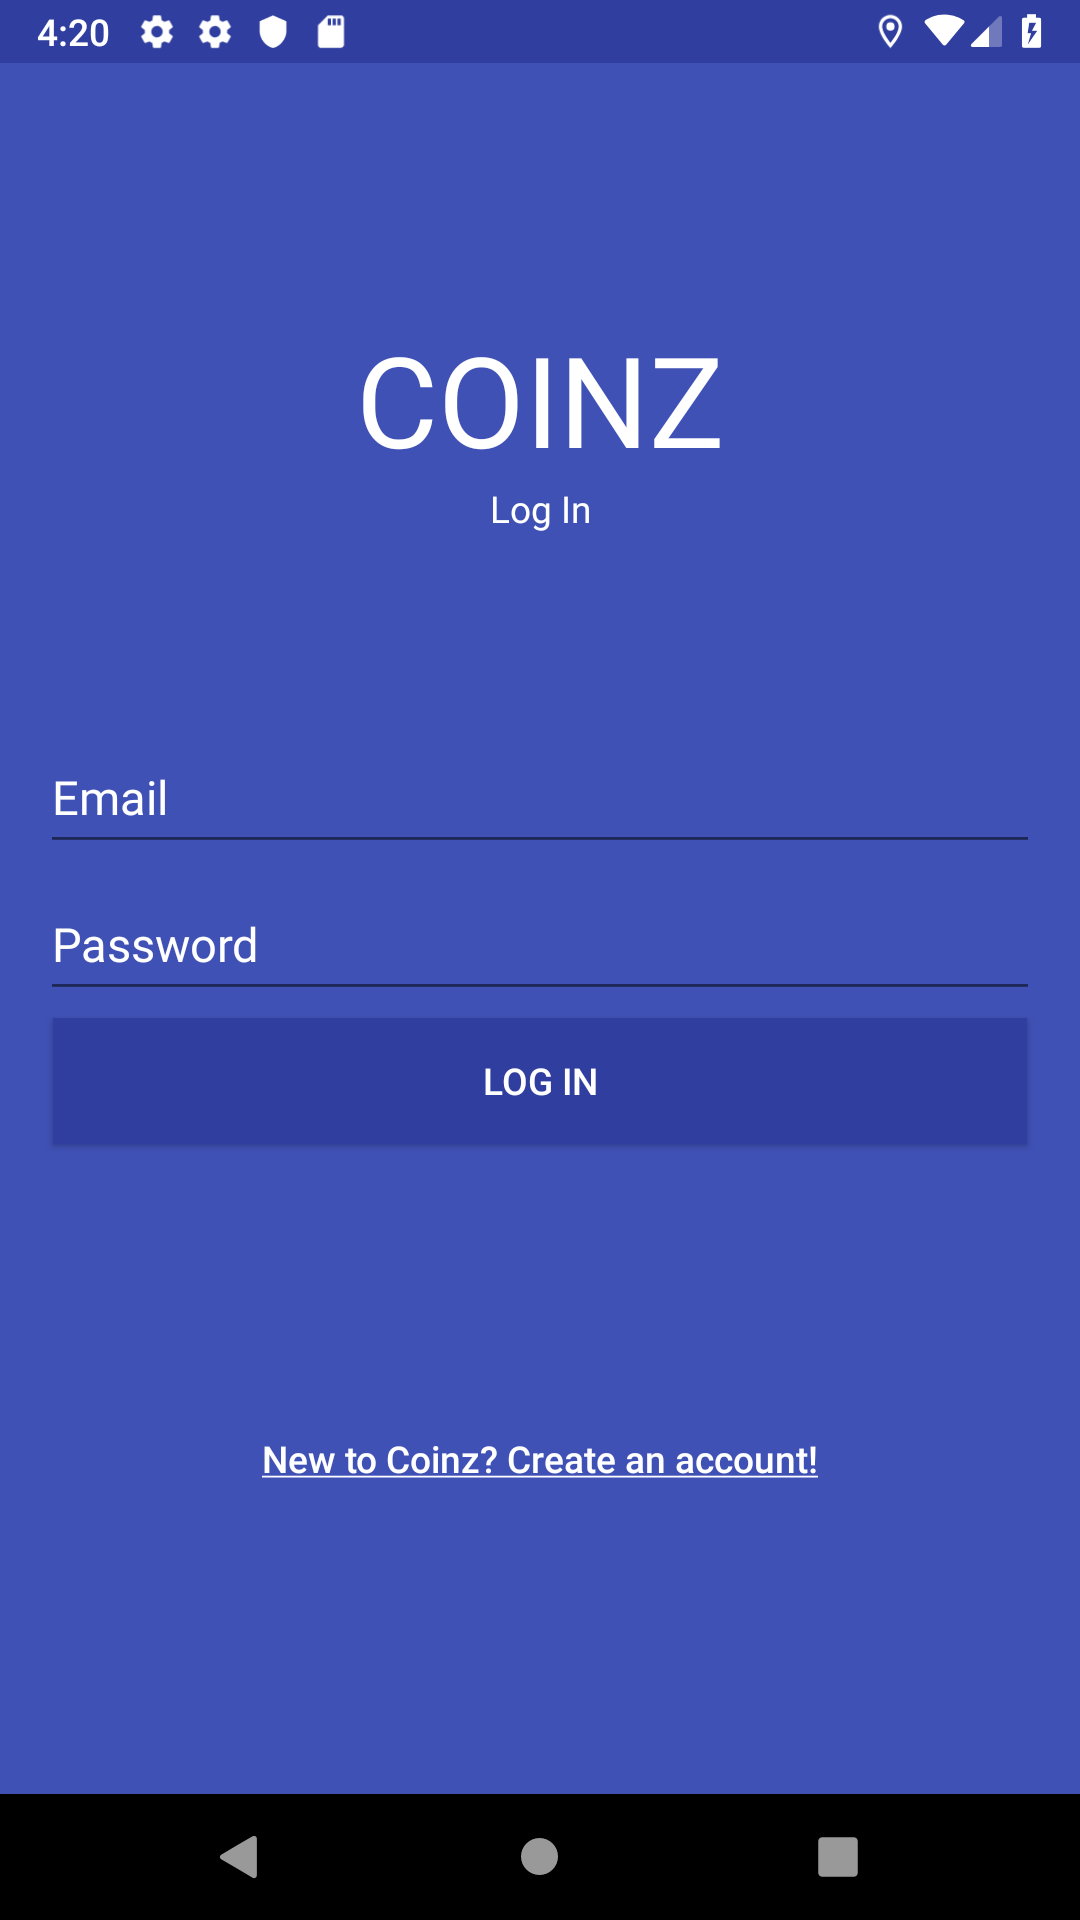
\includegraphics[scale=0.25]{screenshots/log-in/log-in-screen.png}
    \caption{Blank login screen when initially starting the application.}
\end{figure}

    As the user will most likely not have a Coinz user account (managed by Firebase) when they first get the game, they will have to create one, as no user can continue to the actual game without being logged in. To give the user the ability to create an account, there is a link displayed towards the bottom of the login screen which reads "New to Coinz? Create an account!". If the user presses this link (implemented as a button), they are taken to the account creation screen.

\subsection{Onward and Upward - The Account Creation}

    After pressing the link described above, the user is taken to the following screen:

\begin{figure}[H]
    \centering
    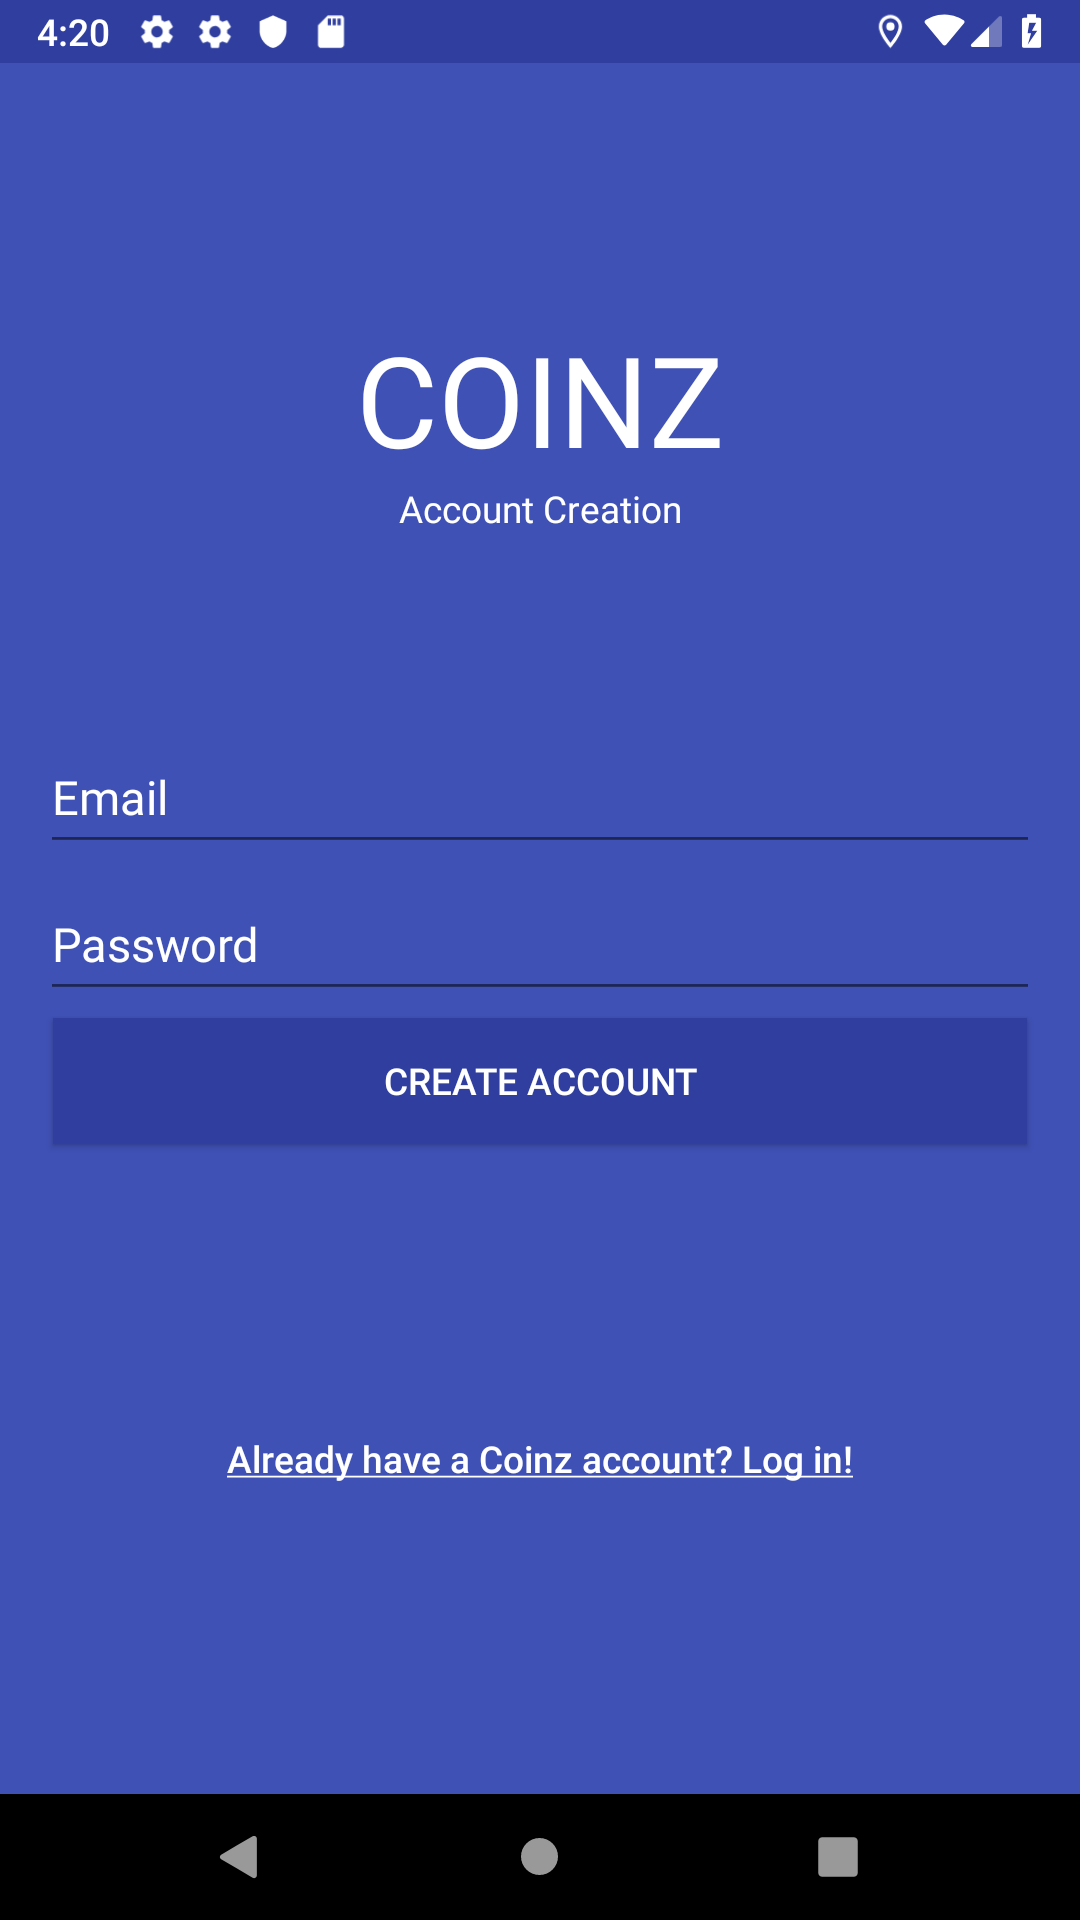
\includegraphics[scale=0.25]{screenshots/account-creation/create-account-screen.png}
    \caption{Blank account creation screen displayed to the user after requesting to create a new account.}
\end{figure}

    The user can now provide their email and password of their choosing:

\begin{figure}[H]
    \centering
    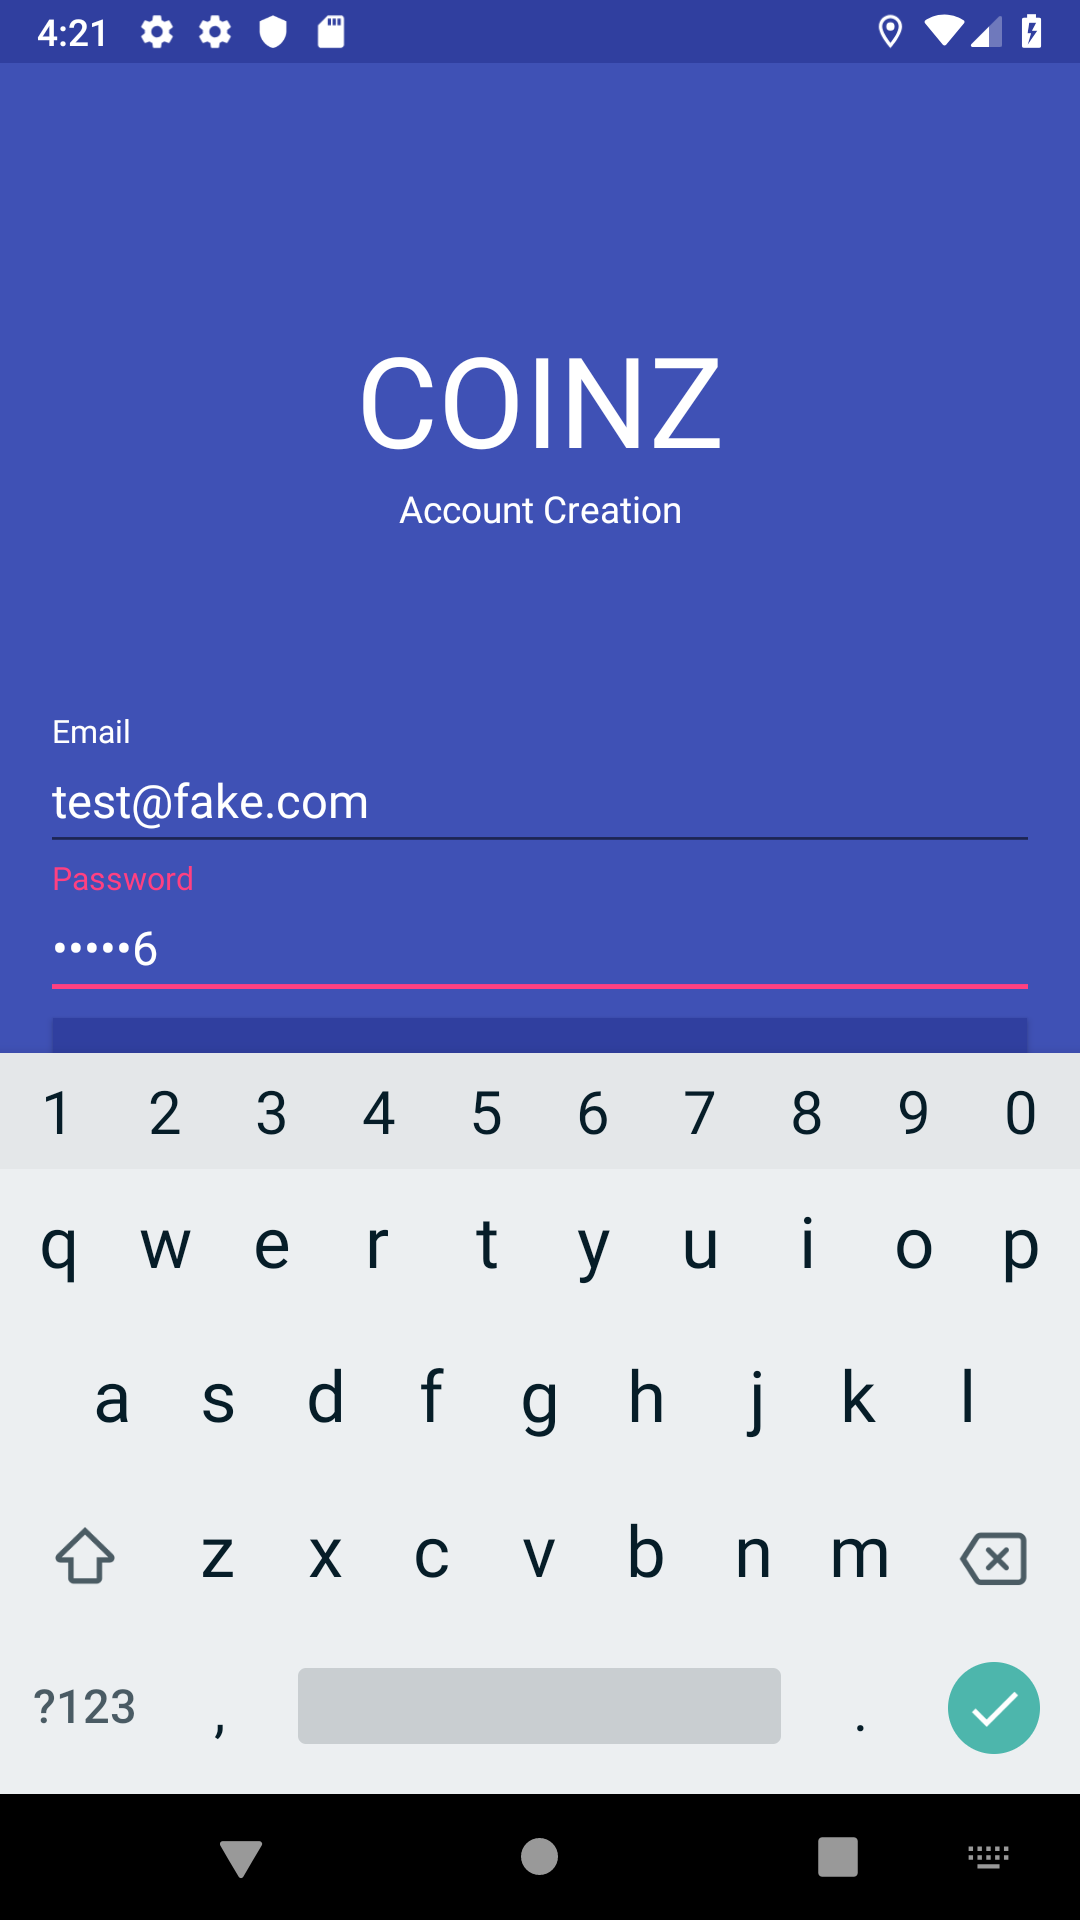
\includegraphics[scale=0.25]{screenshots/account-creation/account-creation-creating-account.png}
    \caption{Test user providing an email address and a password for their new account.}
\end{figure}

    After that is done, the user can create the account by pressing the "Create Account" button. Depending on whether the account creation succeeded or not, the user will be notified with a Toast message with appropriate text as shown below:

\begin{figure}[H]
    \centering
    \begin{minipage}{0.48\textwidth}
        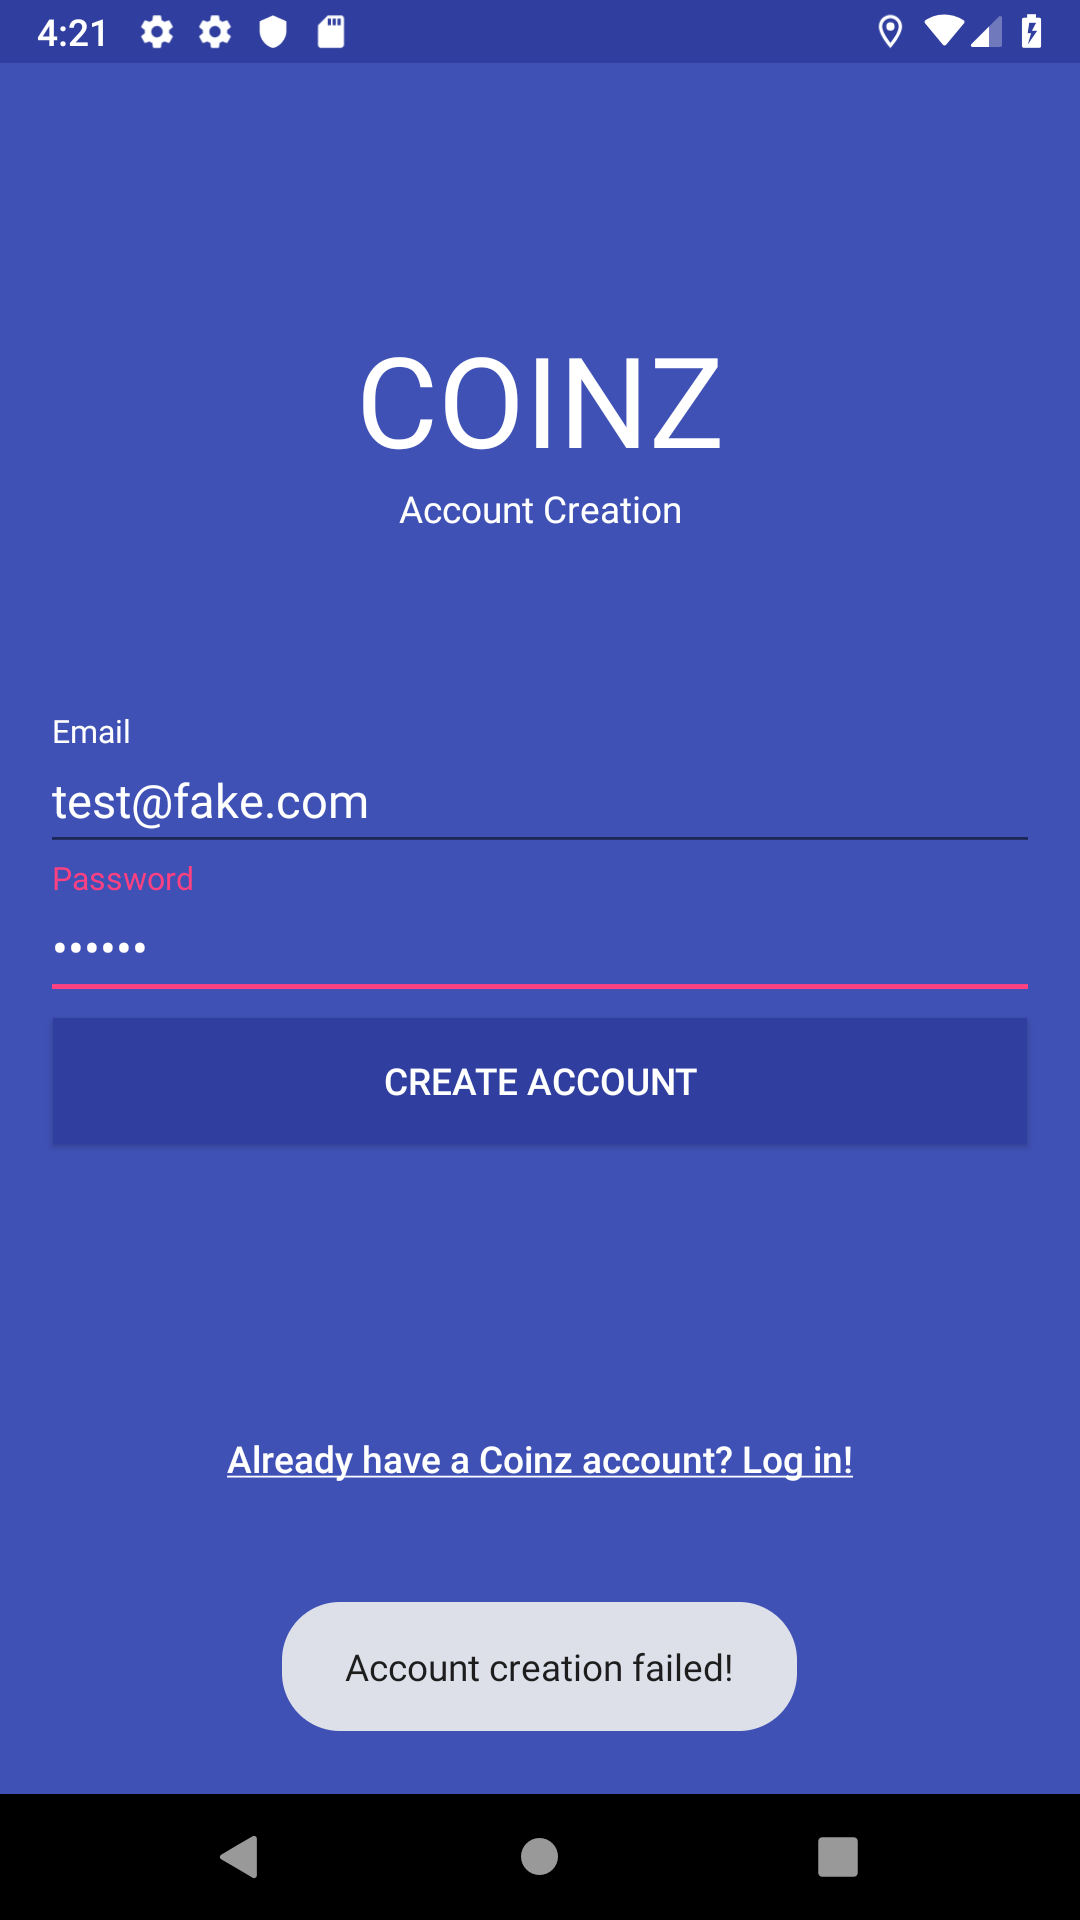
\includegraphics[scale=0.2]{screenshots/account-creation/account-creation-failed.png}
        \caption{Account creation failed.}
    \end{minipage}
    \begin{minipage}{0.48\textwidth}
        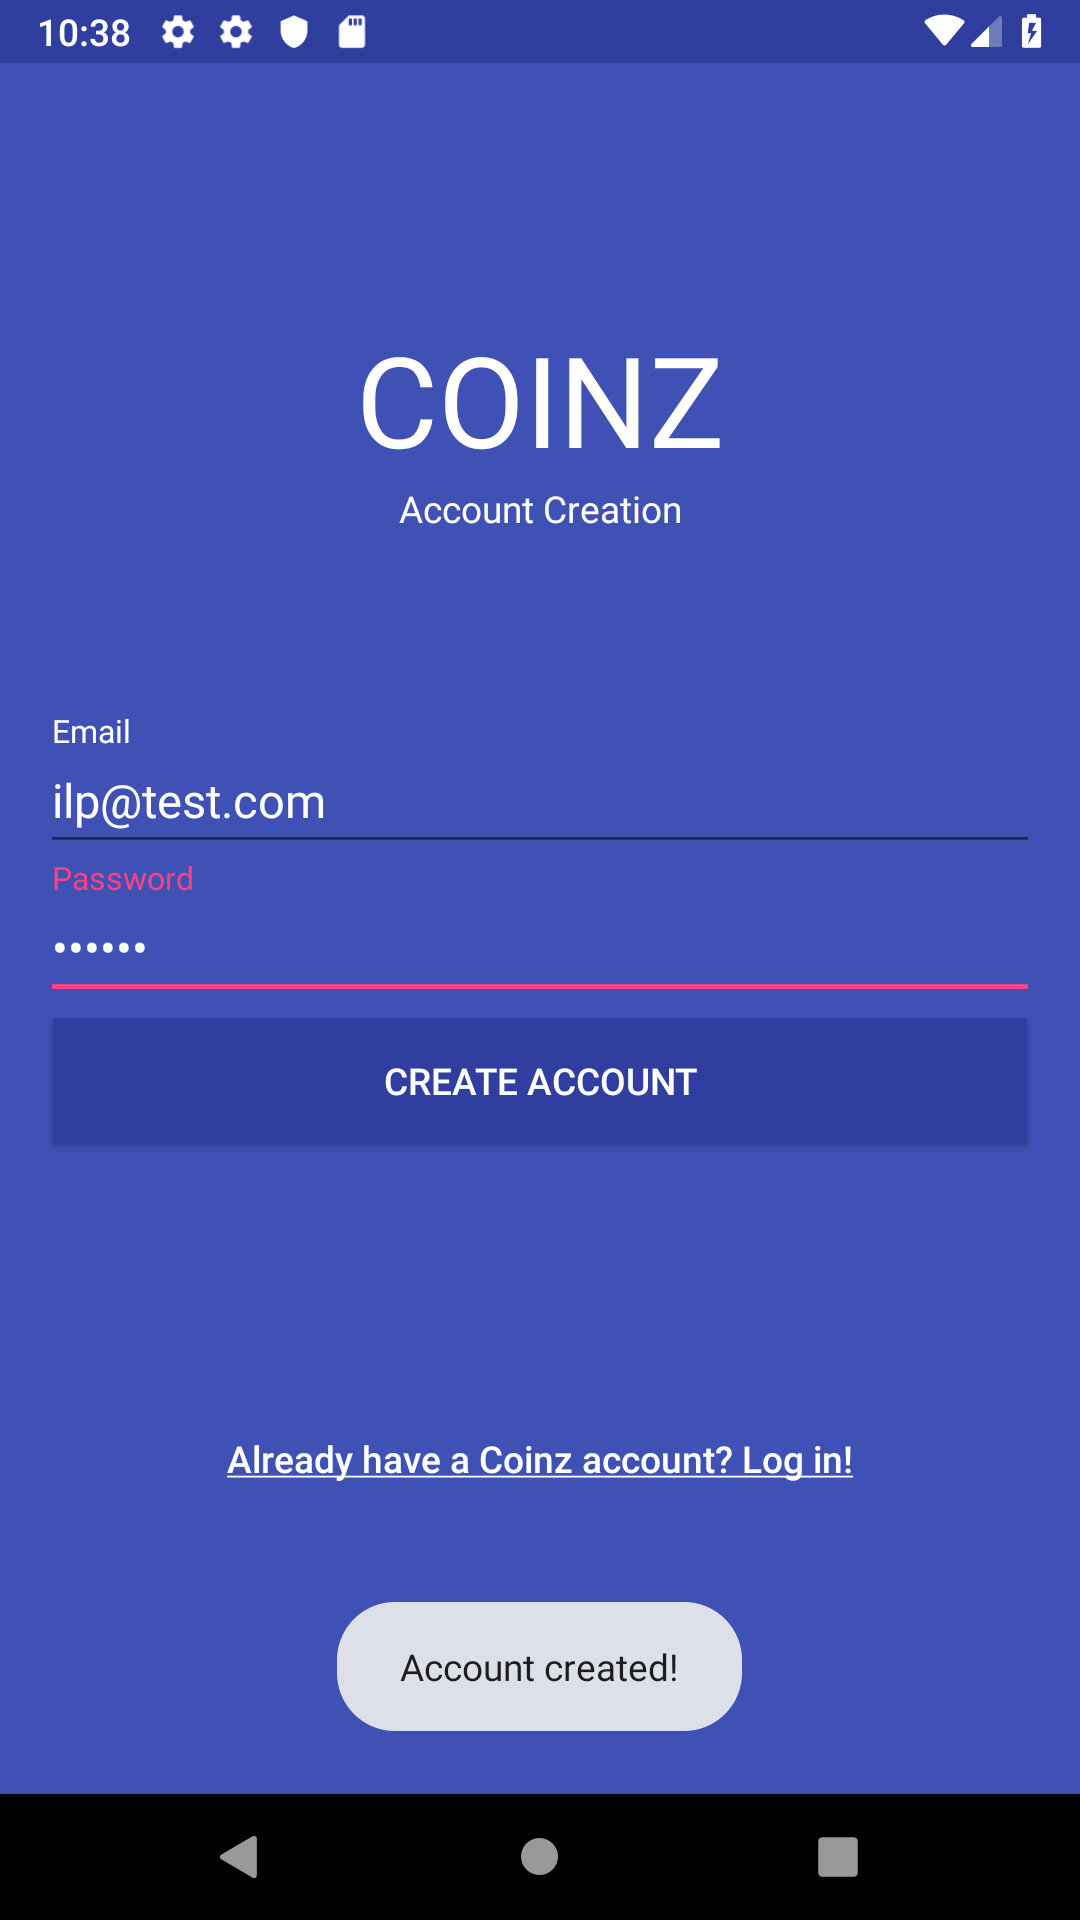
\includegraphics[scale=0.2]{screenshots/account-creation/account-creation-succeeded.png}
        \caption{Account creation succeeded.}
    \end{minipage}
\end{figure}

    The account creation may fail for various reasons, one in particular could be that the data provided by the user is already linked to an existing account. As of the current version of Coinz, the details of the creation failure will not be disclosed to the user. However, if the user account is created successfully, the user is taken straight into the game with the Coinz map in focus.

\subsection{Let the Game(s) Begin - The Coinz Map}

    Since it is the first time the user is playing Coinz, they will not yet have granted the application permissions to access the user's location. Therefore, before going to the actual map, the user will be prompted to grant location access:

\begin{figure}[H]
    \centering
    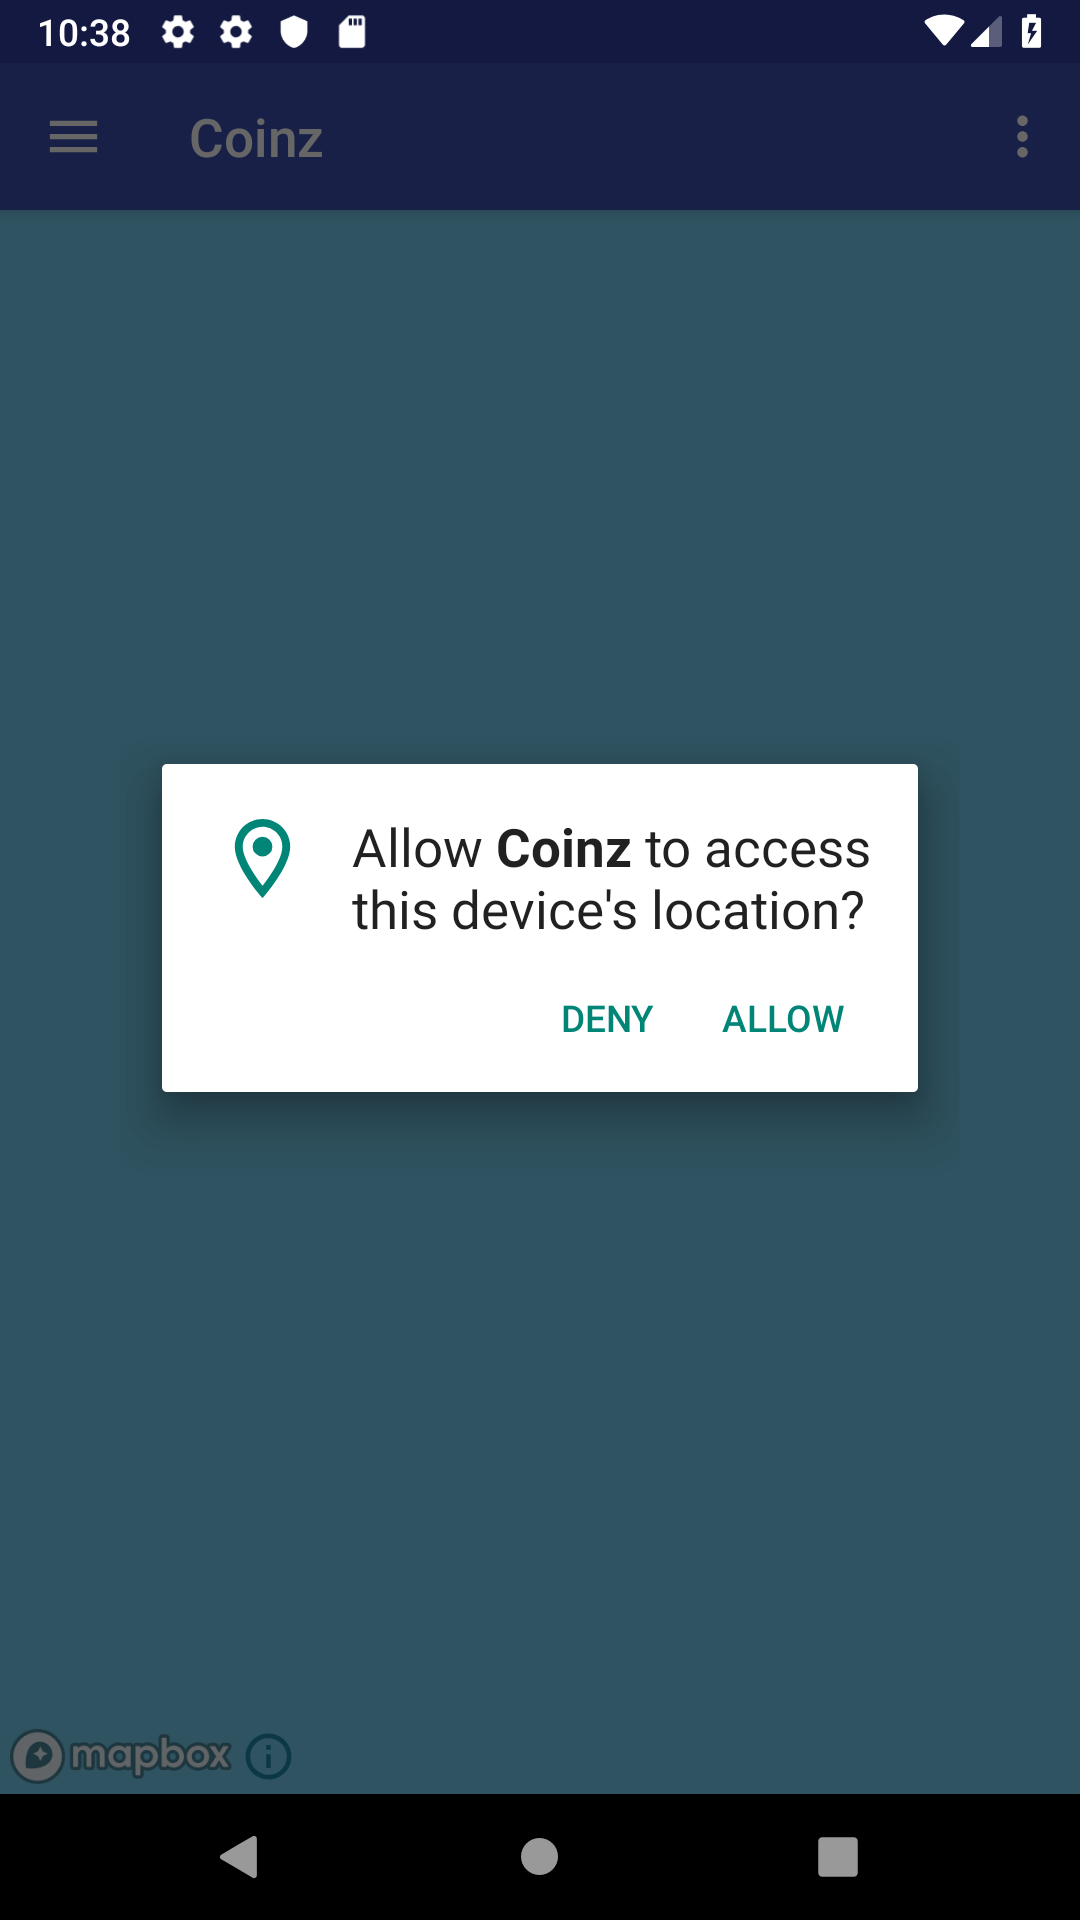
\includegraphics[scale=0.25]{screenshots/map/asking-for-permissions.png}
    \caption{User being prompted to provide the required location access permission.}
\end{figure}

    Once that is taken care of, the user location will be pulled from the device and updated on the screen, finally showing the name-giving coins as markers on the map:

\begin{figure}[H]
    \centering
    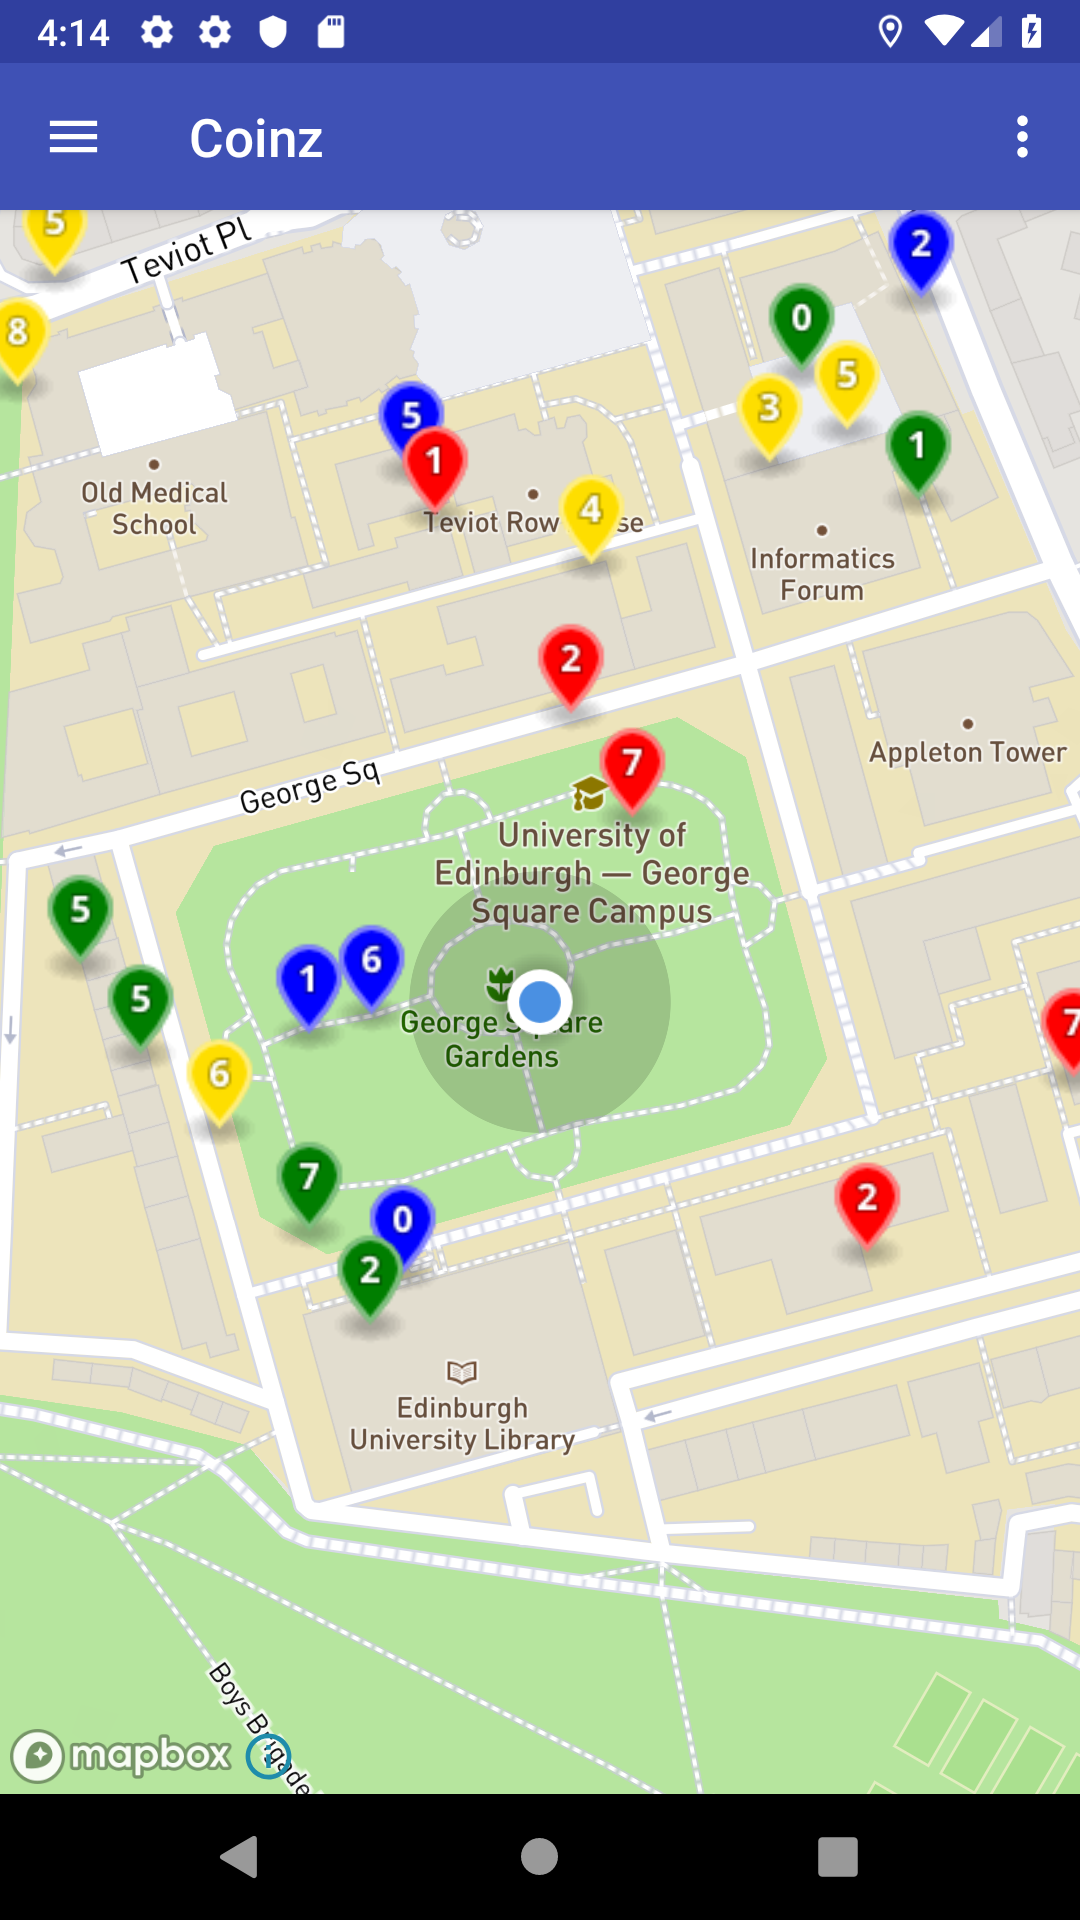
\includegraphics[scale=0.25]{screenshots/map/map-with-markers.png}
    \caption{A first look at a map with coin markers.}
\end{figure}

    There is currently no tutorial implemented, so the user will essentially have to figure out how to play on their own. It is not too hard though, it will quickly become apparent that the user will have to press on a marker to open a collection dialog:

\begin{figure}[H]
    \centering
    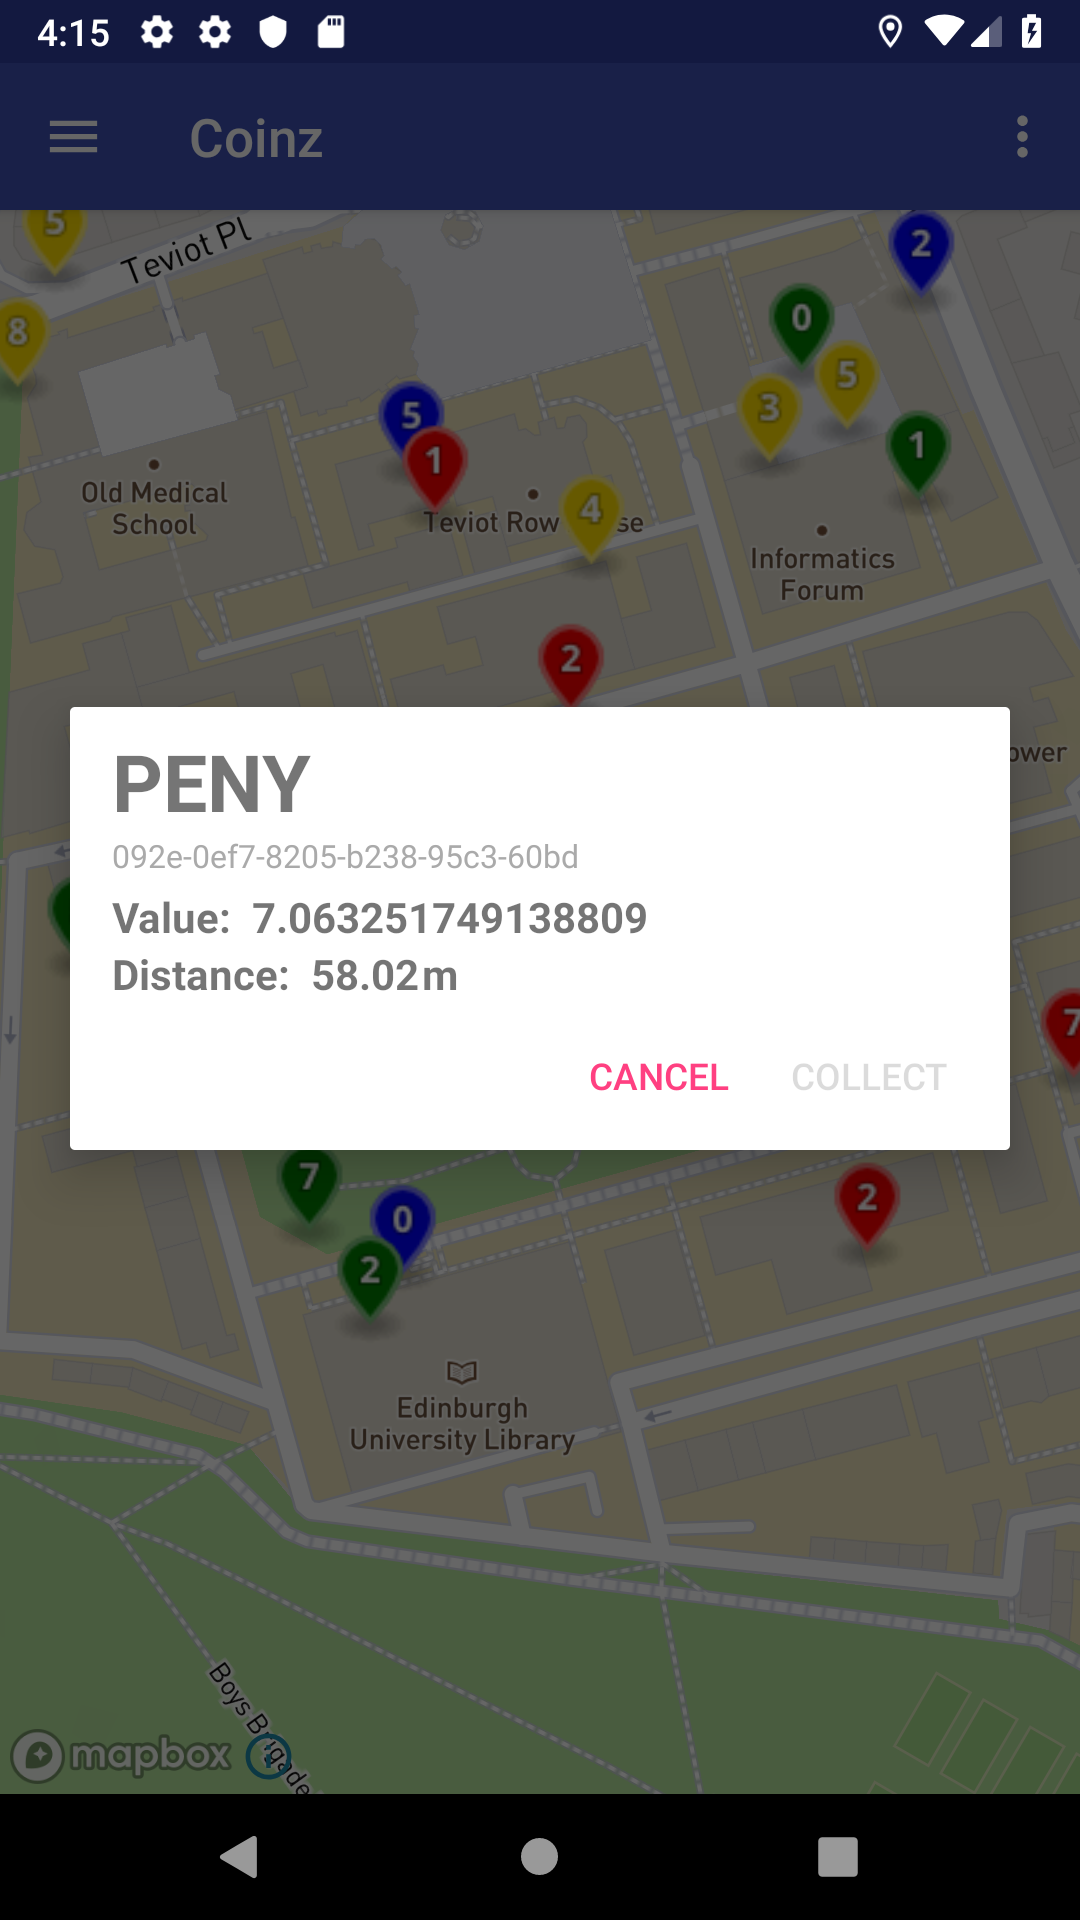
\includegraphics[scale=0.25]{screenshots/map/coin-collect-dialog-too-far.png}
    \caption{A typical coin collection dialog. Information displayed: the currency of the coin, its ID, the coin value and the user's distance to the coin in meters.}
\end{figure}

    In this particular instance the user is too far away from the coin to collect it. This is shown by the "Collect" button being disabled for the user, as can be seen in the image above by the fact that the "Collect" button is grayed-out.

    In order to collect a coin, the user must be within at least 25 meters of the coin on the map, in which case the "Collect" button will become active:

\begin{figure}[H]
    \centering
    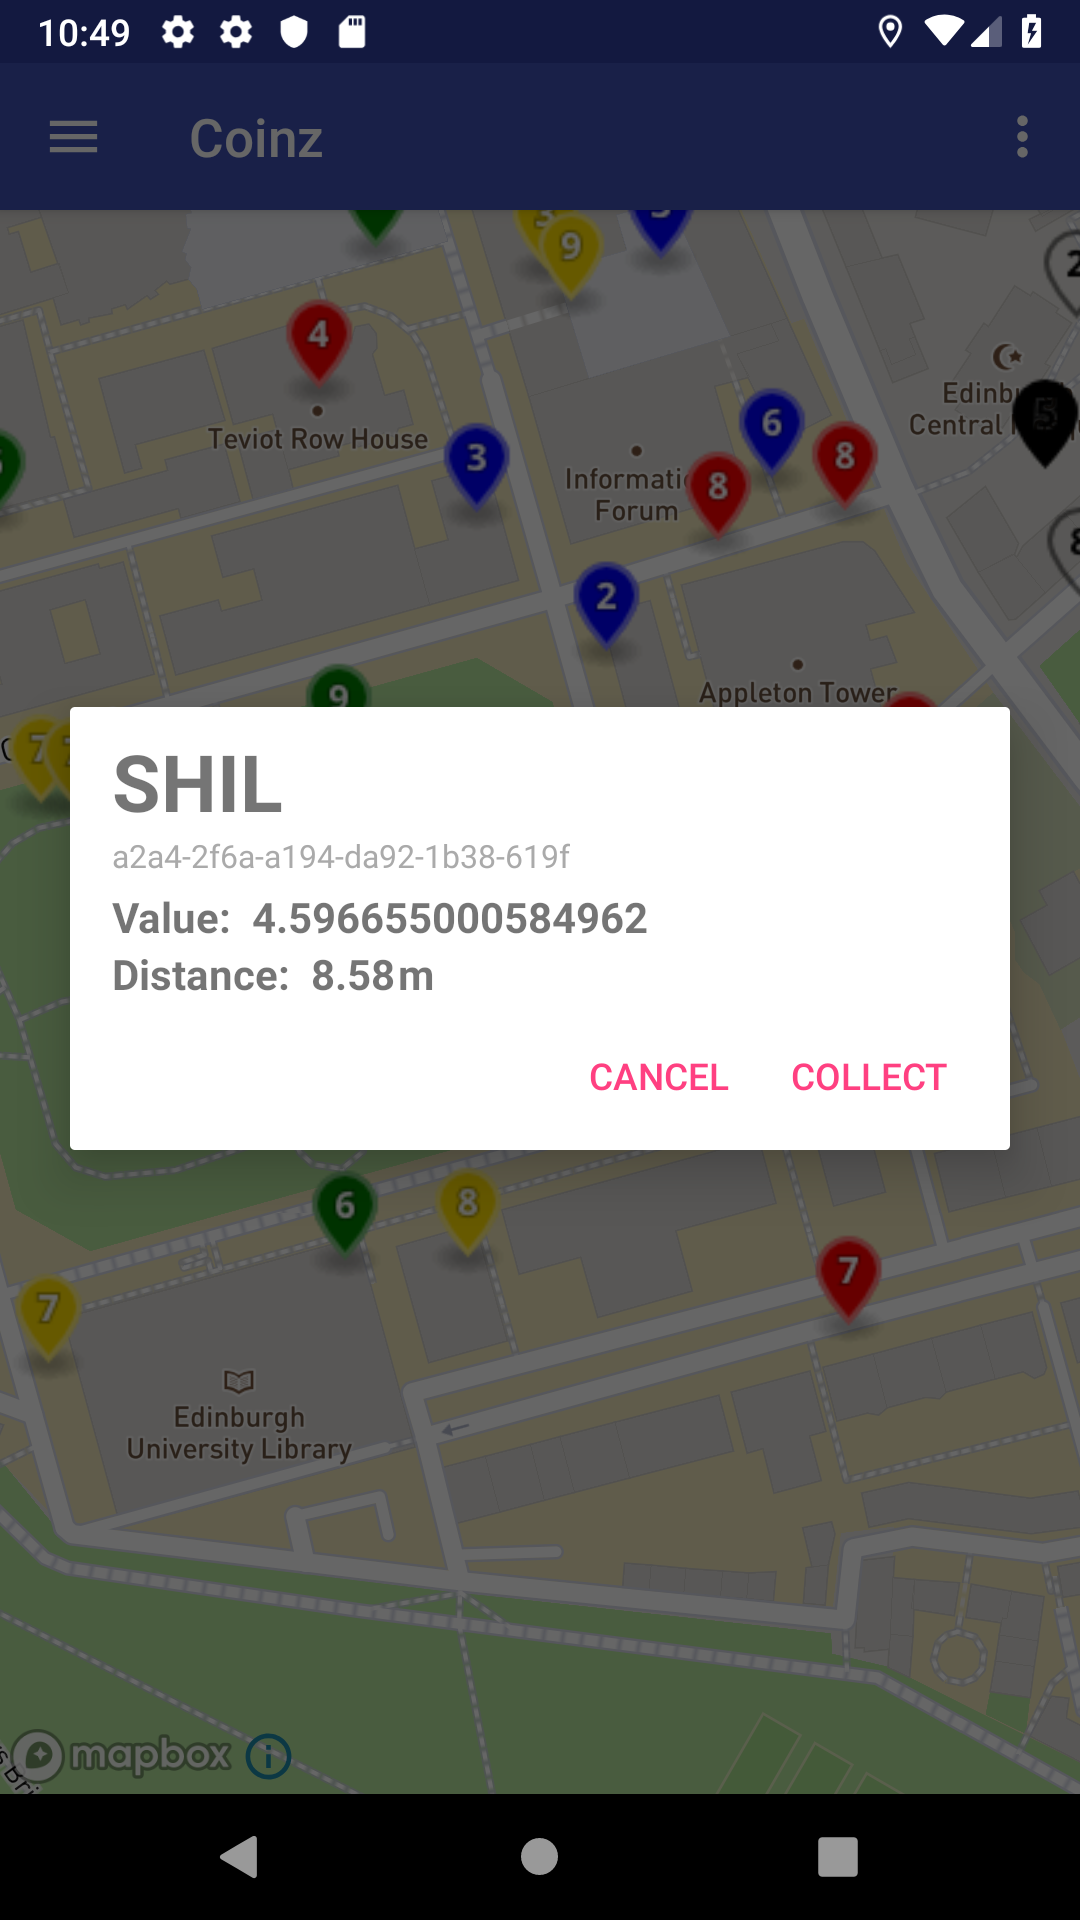
\includegraphics[scale=0.25]{screenshots/map/collect-coin-in-range.png}
    \caption{User is within 25 meters of the coin they clicked on.}
\end{figure}

    If they so choose, they can now collect the coin, in which case the marker will disappear from the map and the coin will wander into the user's Local Wallet. Before we go on to explore the Local Wallet, however, there are two caveats to collecting coins, namely the two bonus features.

%\begin{figure}[H]
%    \centering
%    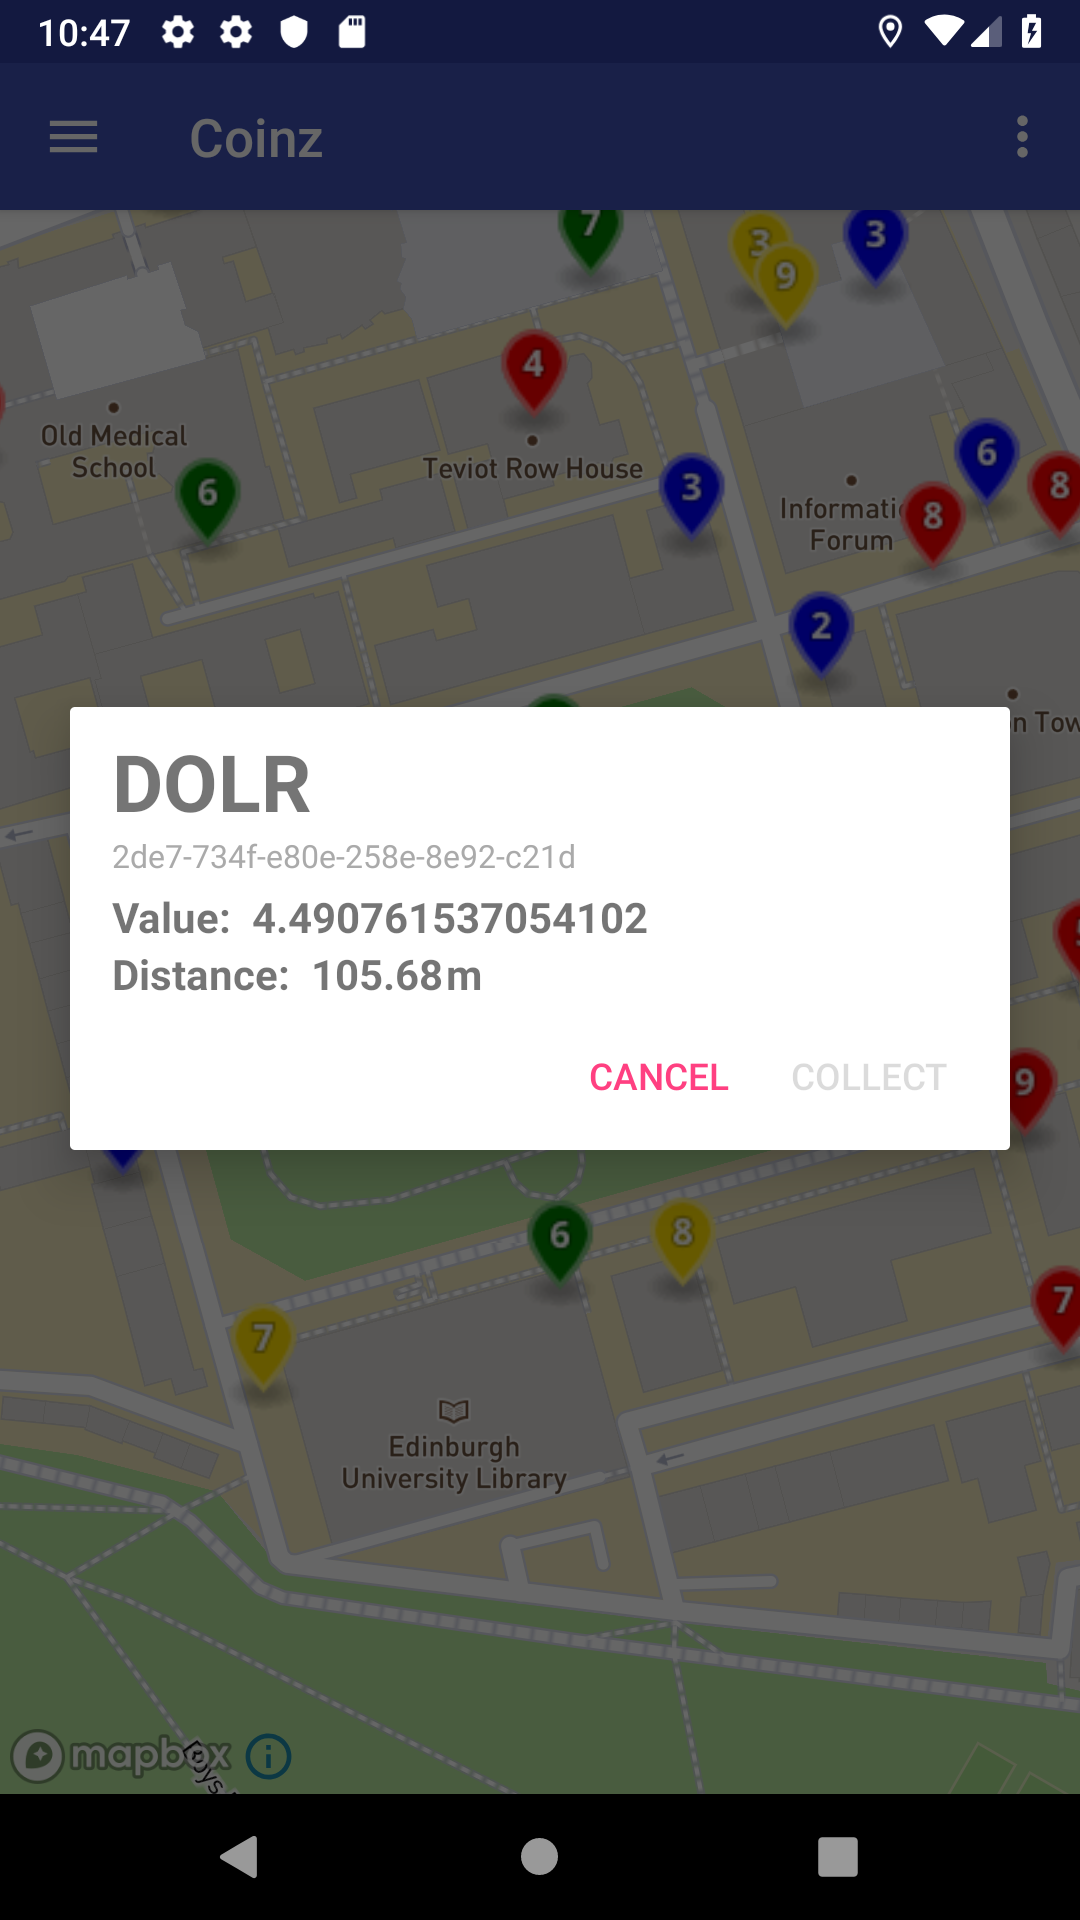
\includegraphics[scale=0.12]{screenshots/map/collect-coin-no-multipliers.png}
%    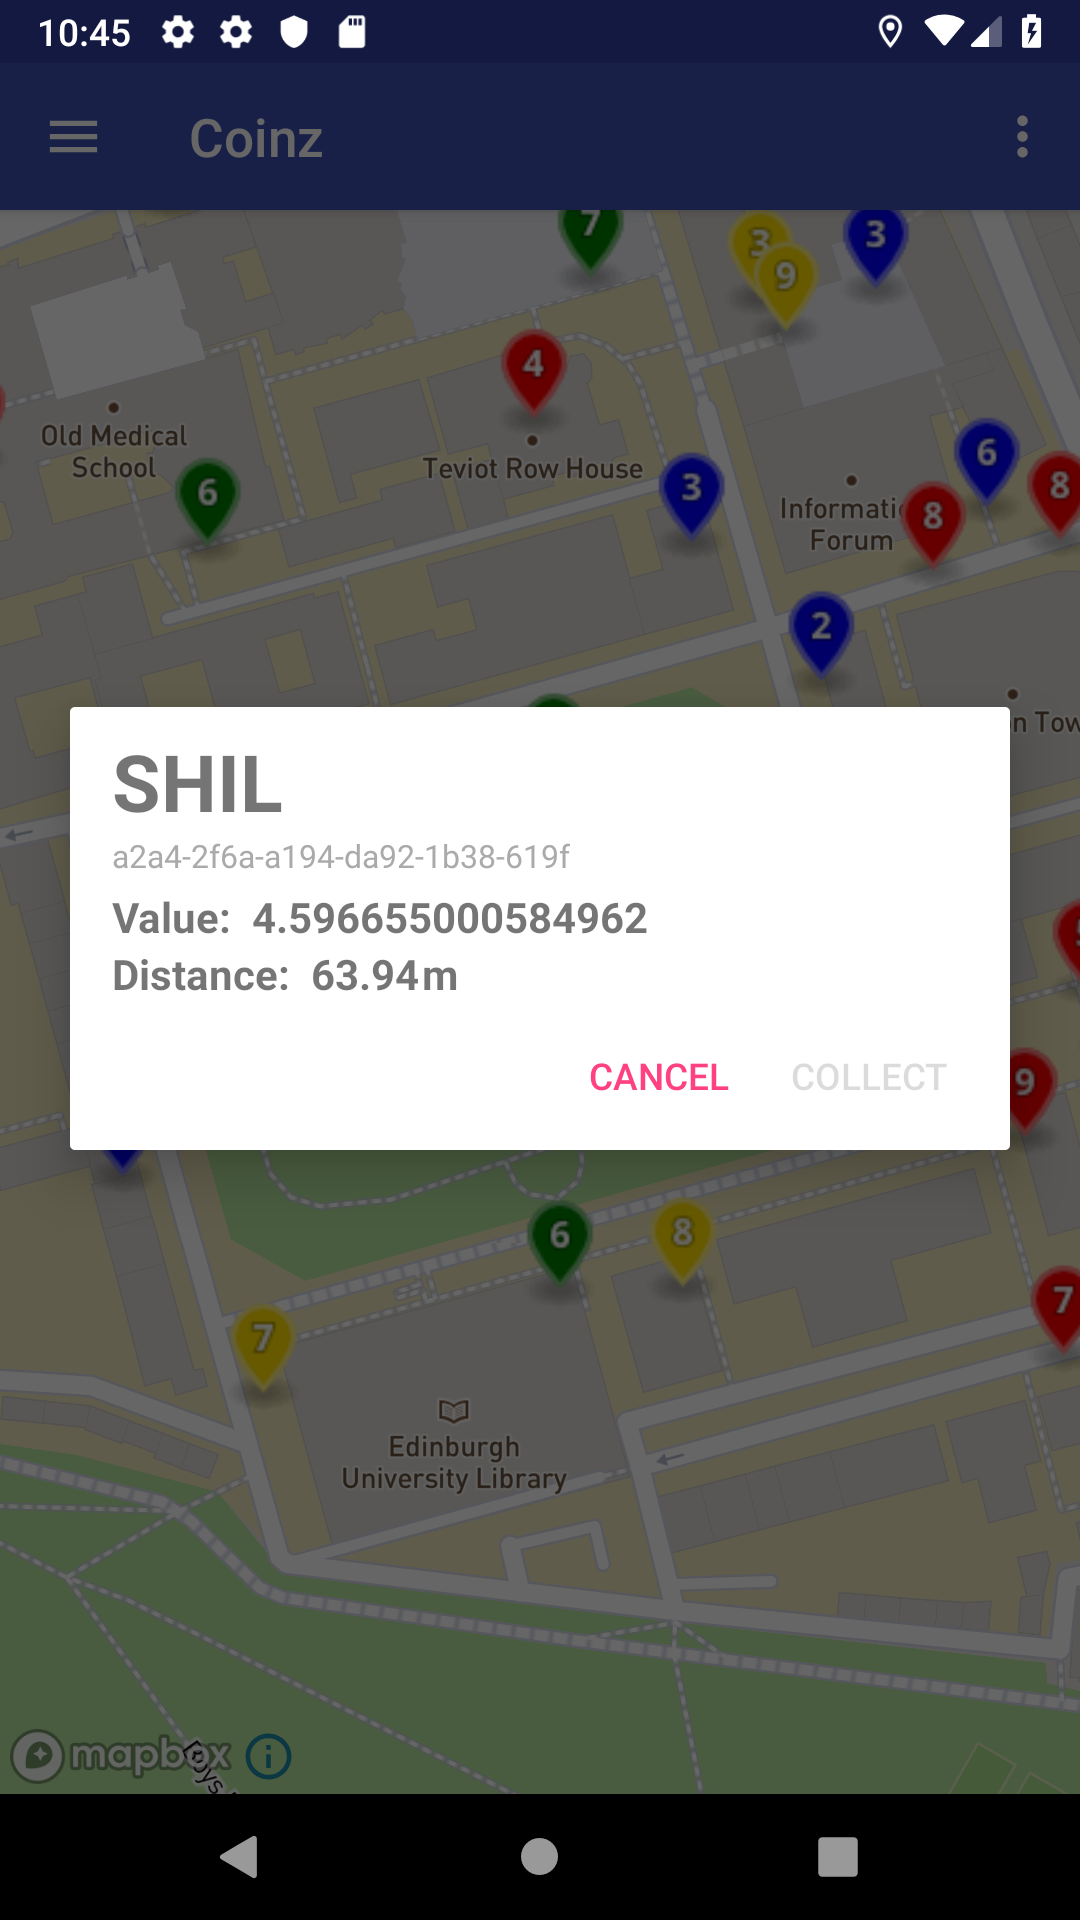
\includegraphics[scale=0.12]{screenshots/map/collect-coin-no-symbol-multiplier-color-multiplier.png}
%    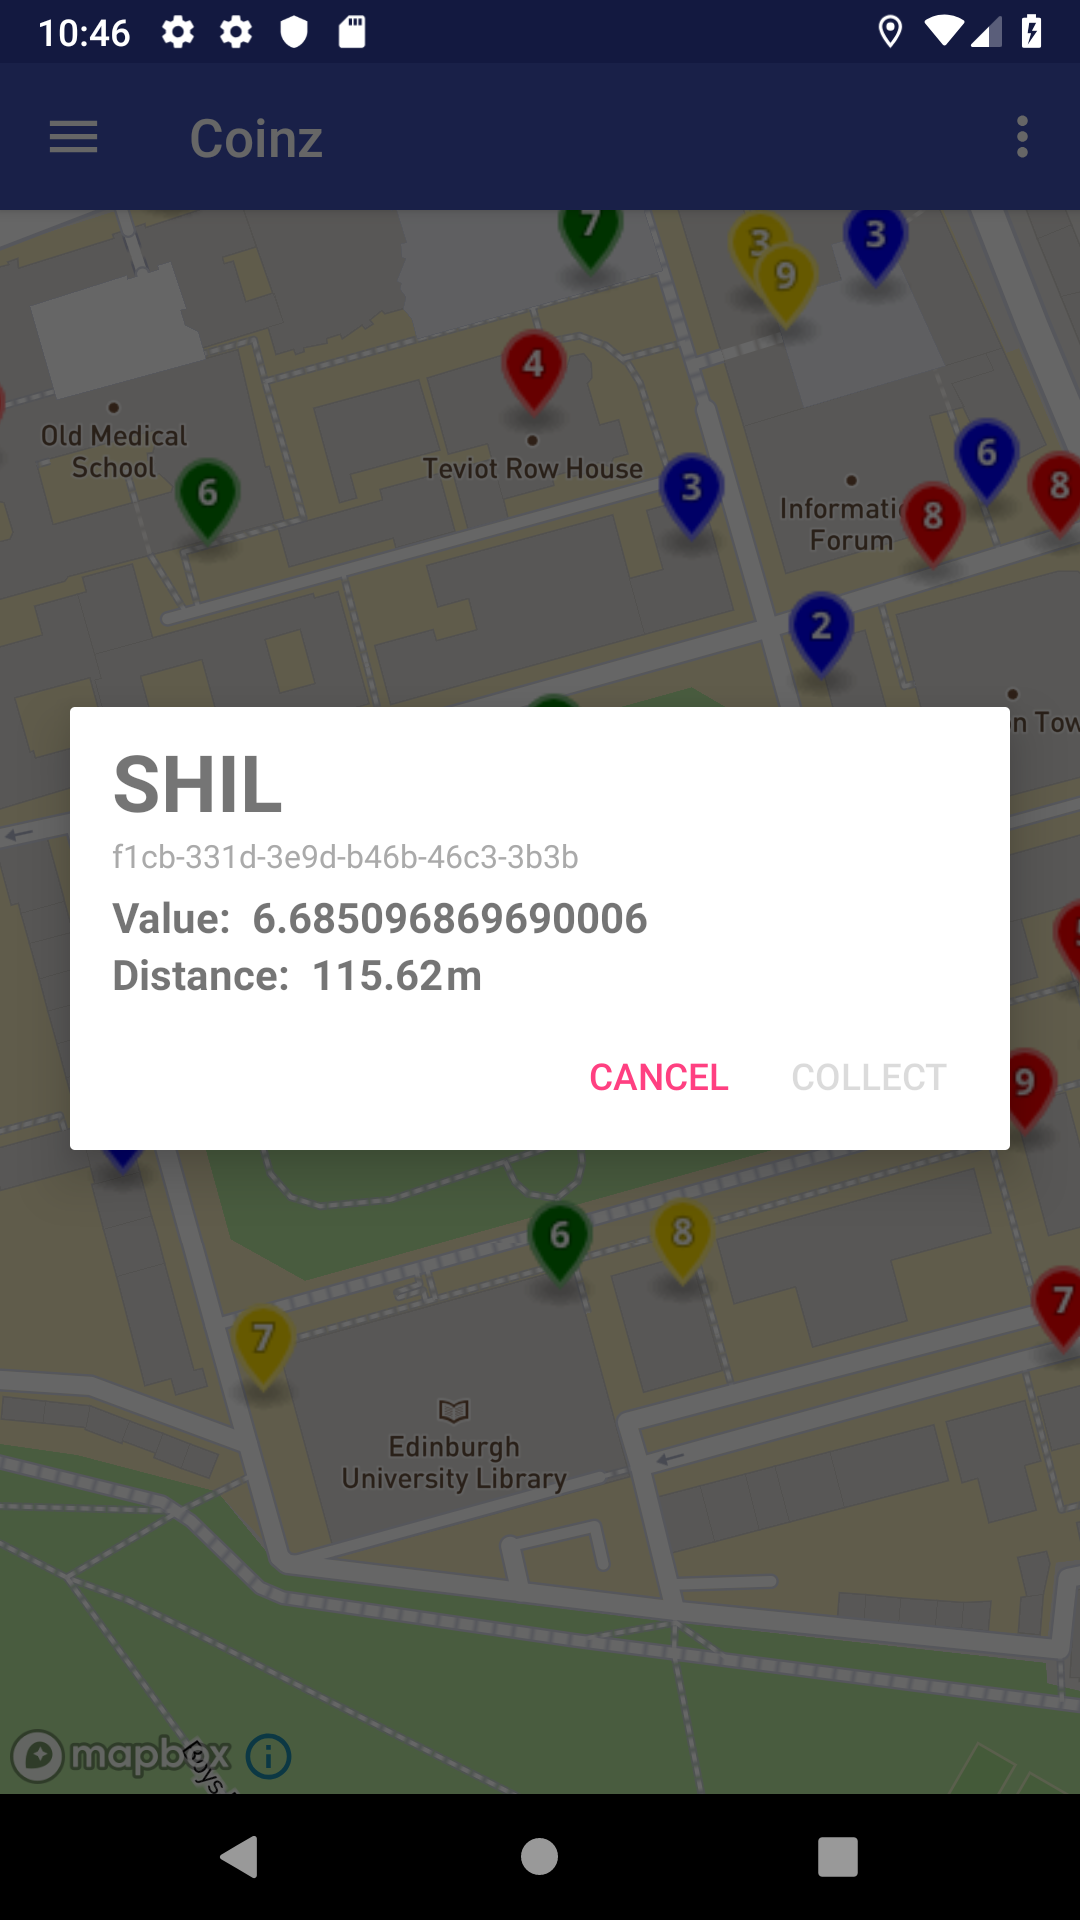
\includegraphics[scale=0.12]{screenshots/map/collect-coin-symbol-and-color-multipliers.png}
%    \caption{Left: A coin with not a single multiplier applied to it. Middle: A coin with only a marker color multiplier applied to it. Right: A coin will both a marker color and marker symbol multiplier applied to it. Notice the relative value range differences.}
%\end{figure}

    While not implemented with a visual indicator within the interface, the bonus feature multipliers act on the value of the coin while it is being transferred from the map to the Local Wallet. Given the right conditions, the coin value that is displayed in the above dialogues will be multiplied and then stored in the Local Wallet.

\subsection{Thinking Outside the (Map)Box - The Local Wallet}

    Once coins have been collected, they are transferred into the user's Local Wallet where they can have a look at their achievements so far. To get to the Local Wallet, the user needs to open the navigation drawer:

\begin{figure}[H]
    \centering
    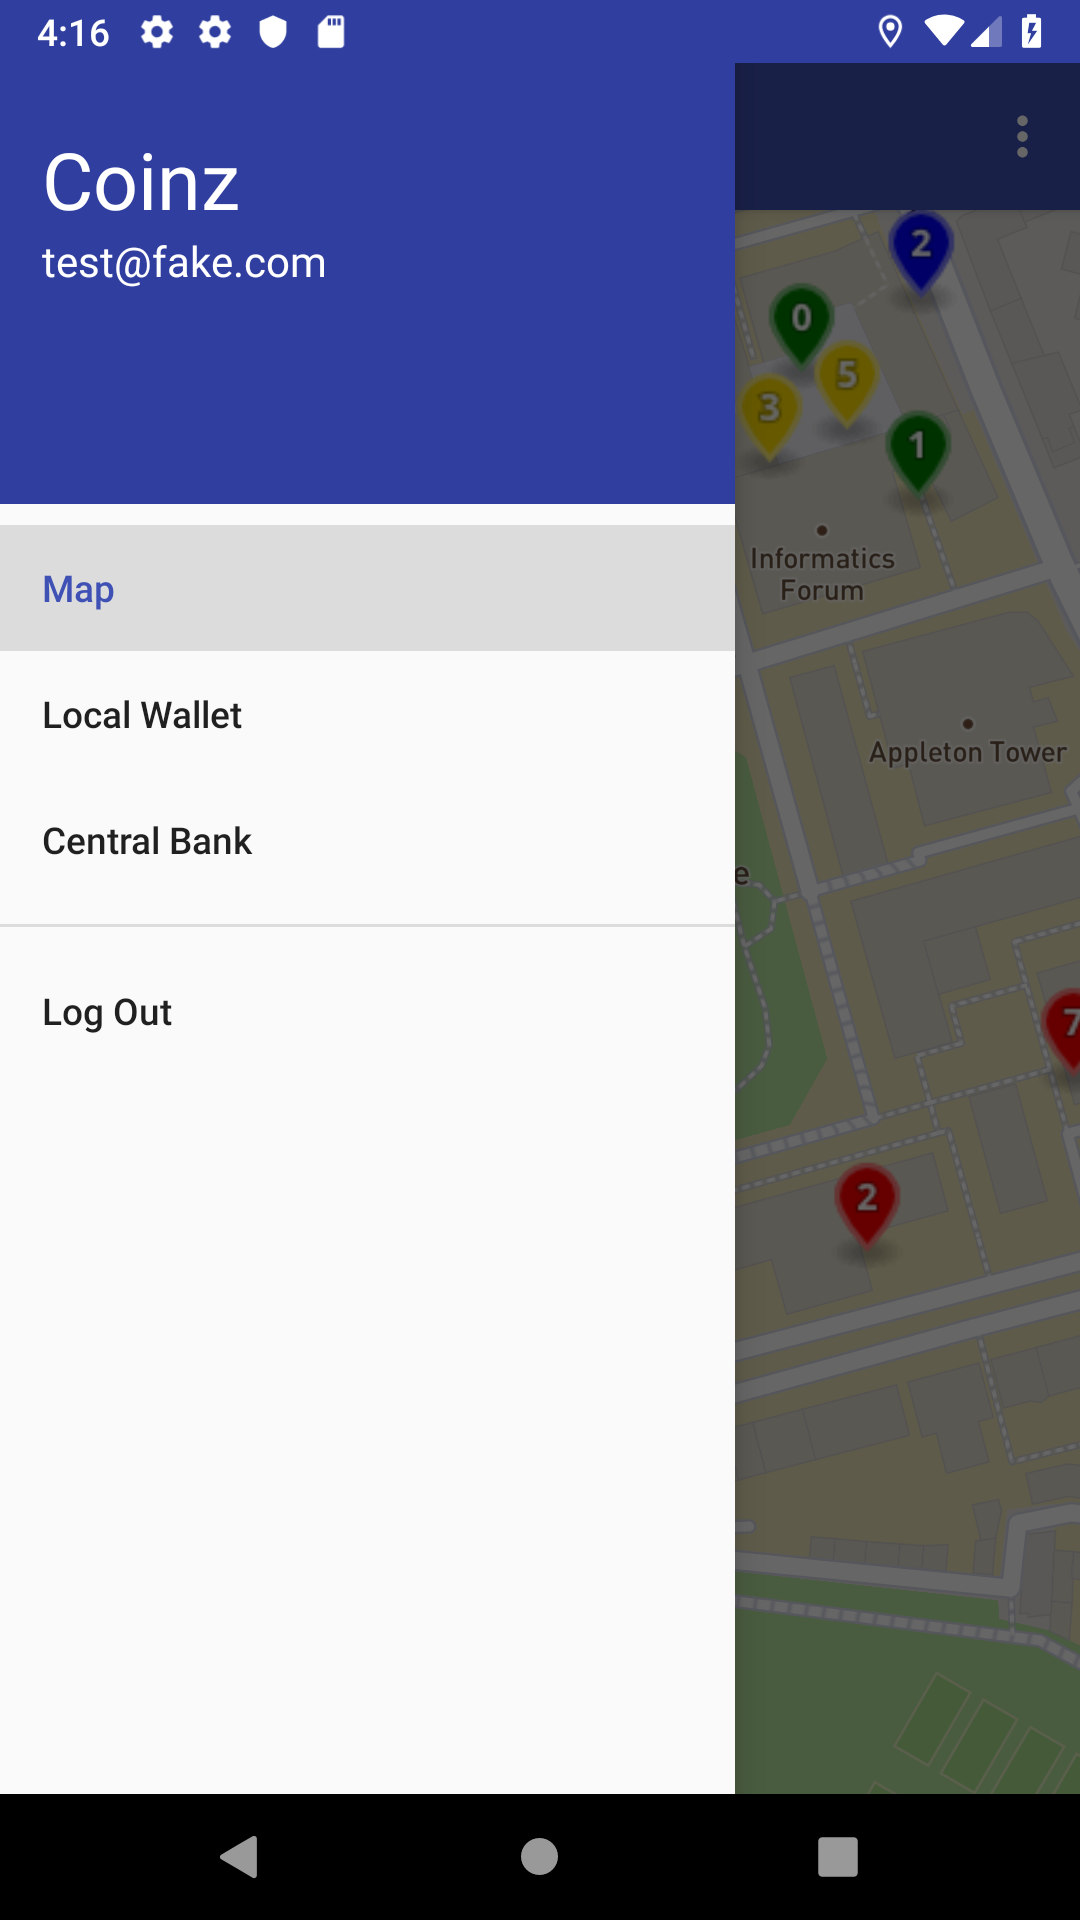
\includegraphics[scale=0.25]{screenshots/navigation-drawer/navigation-drawer-map-selected.png}
    \caption{Navigation drawer as the central place to switch between different app features. User's email used to log in is displayed at the top.}
\end{figure}

    If the user now clicks on the Local Wallet it will change from the map view to the wallet view. Initially, when the user has not collected any coins yet \emph{on that day}, the Local Wallet will be empty:

\begin{figure}[H]
    \centering
    \begin{minipage}[t]{0.48\textwidth}
        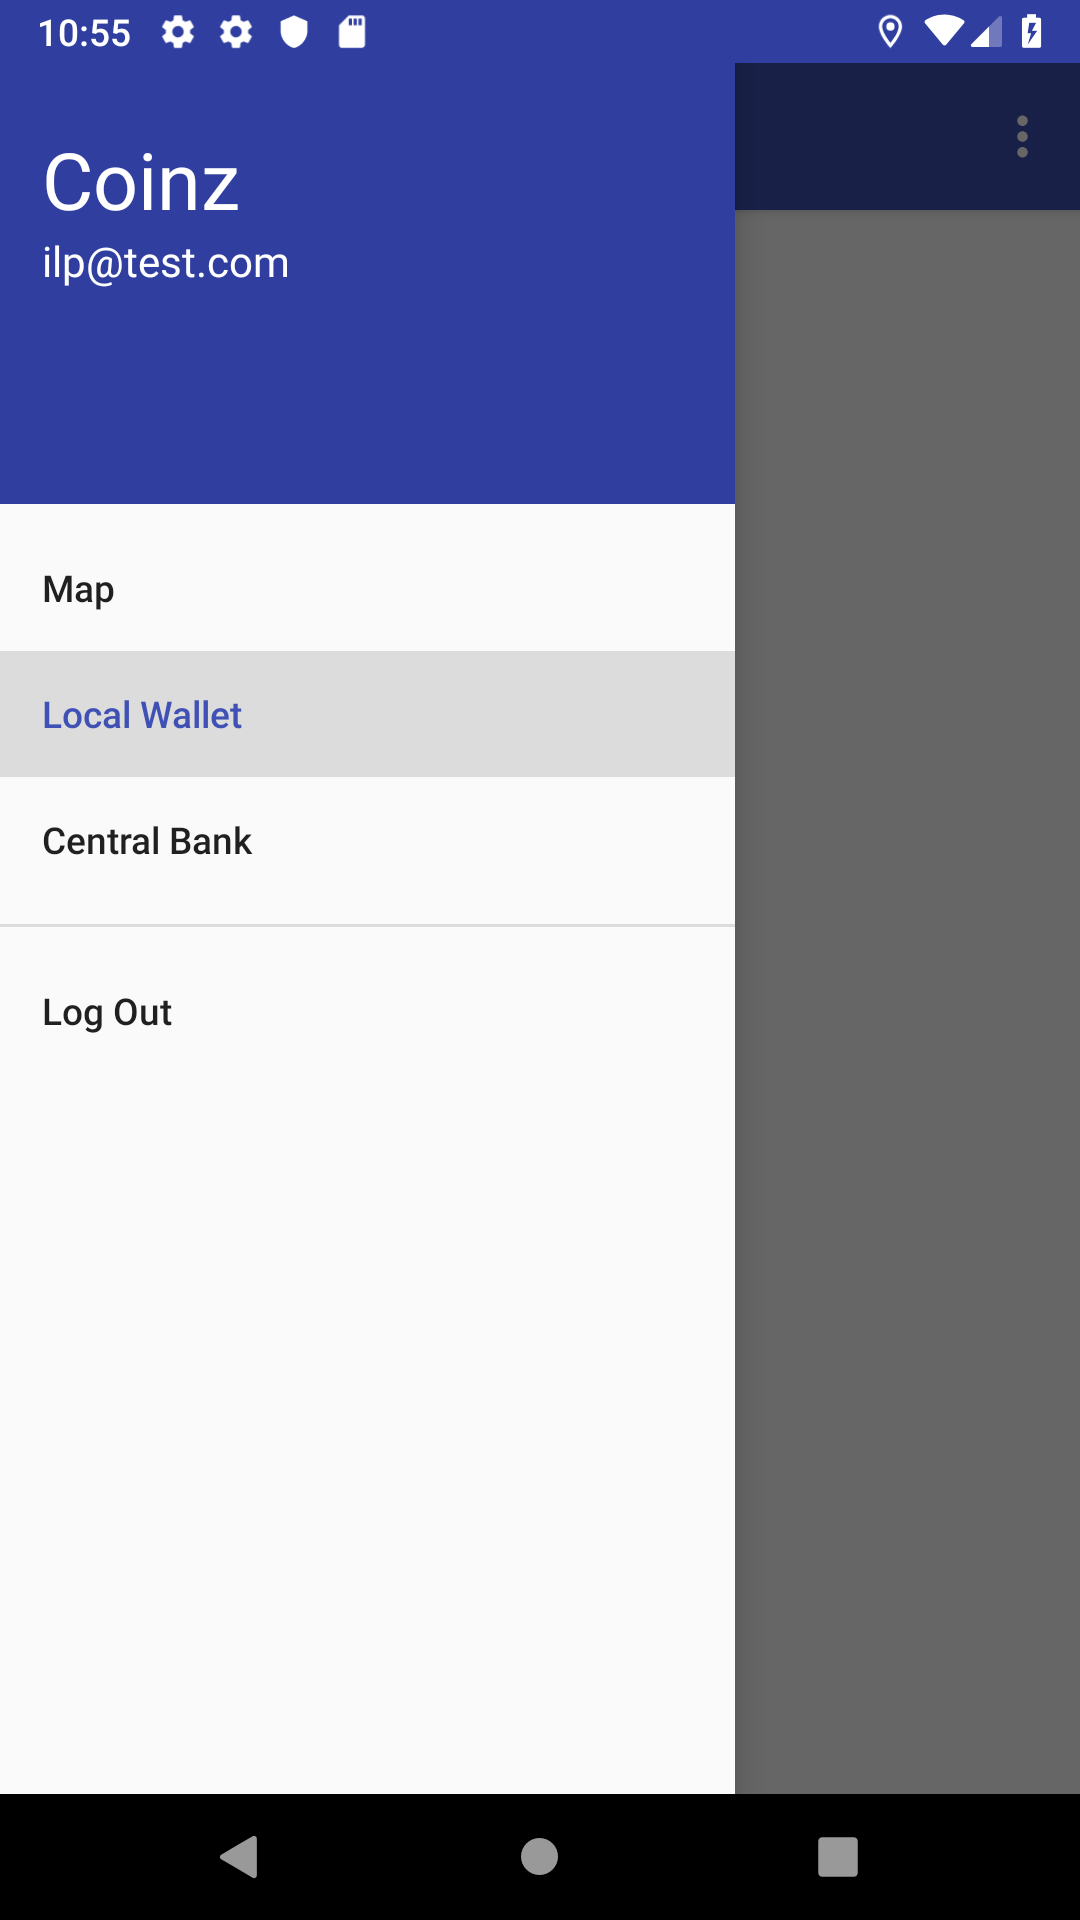
\includegraphics[scale=0.2]{screenshots/local-wallet/selected-empty-local-wallet.png}
        \caption{Selecting the Local Wallet in the navigation drawer.}
    \end{minipage}
    \begin{minipage}[t]{0.48\textwidth}
        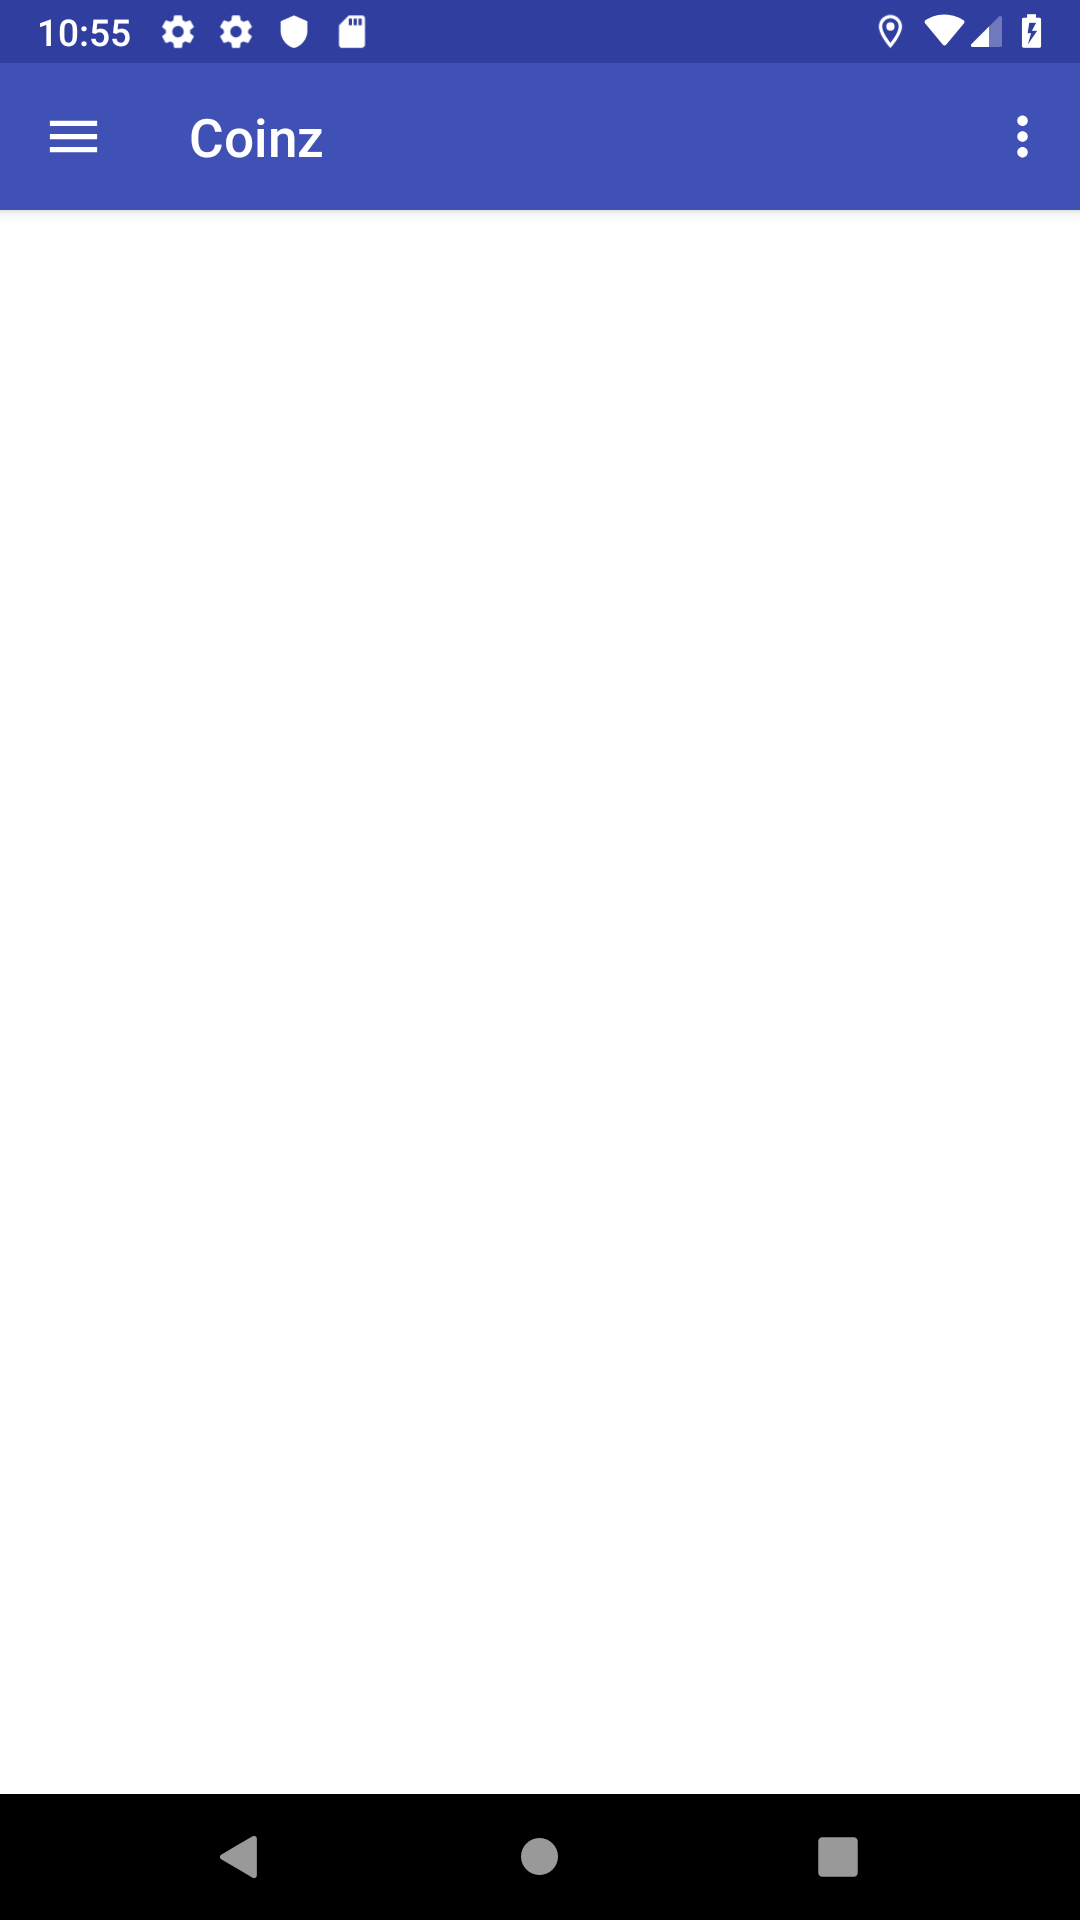
\includegraphics[scale=0.2]{screenshots/local-wallet/empty-local-wallet.png}
        \caption{Initially empty Local Wallet.}
    \end{minipage}
\end{figure}

    Now, as the user plays the game, the Local Wallet will fill with lots of wonderful coins which are all listed within the Local Wallet, with some key information about them displayed as well:

\begin{figure}[H]
    \centering
    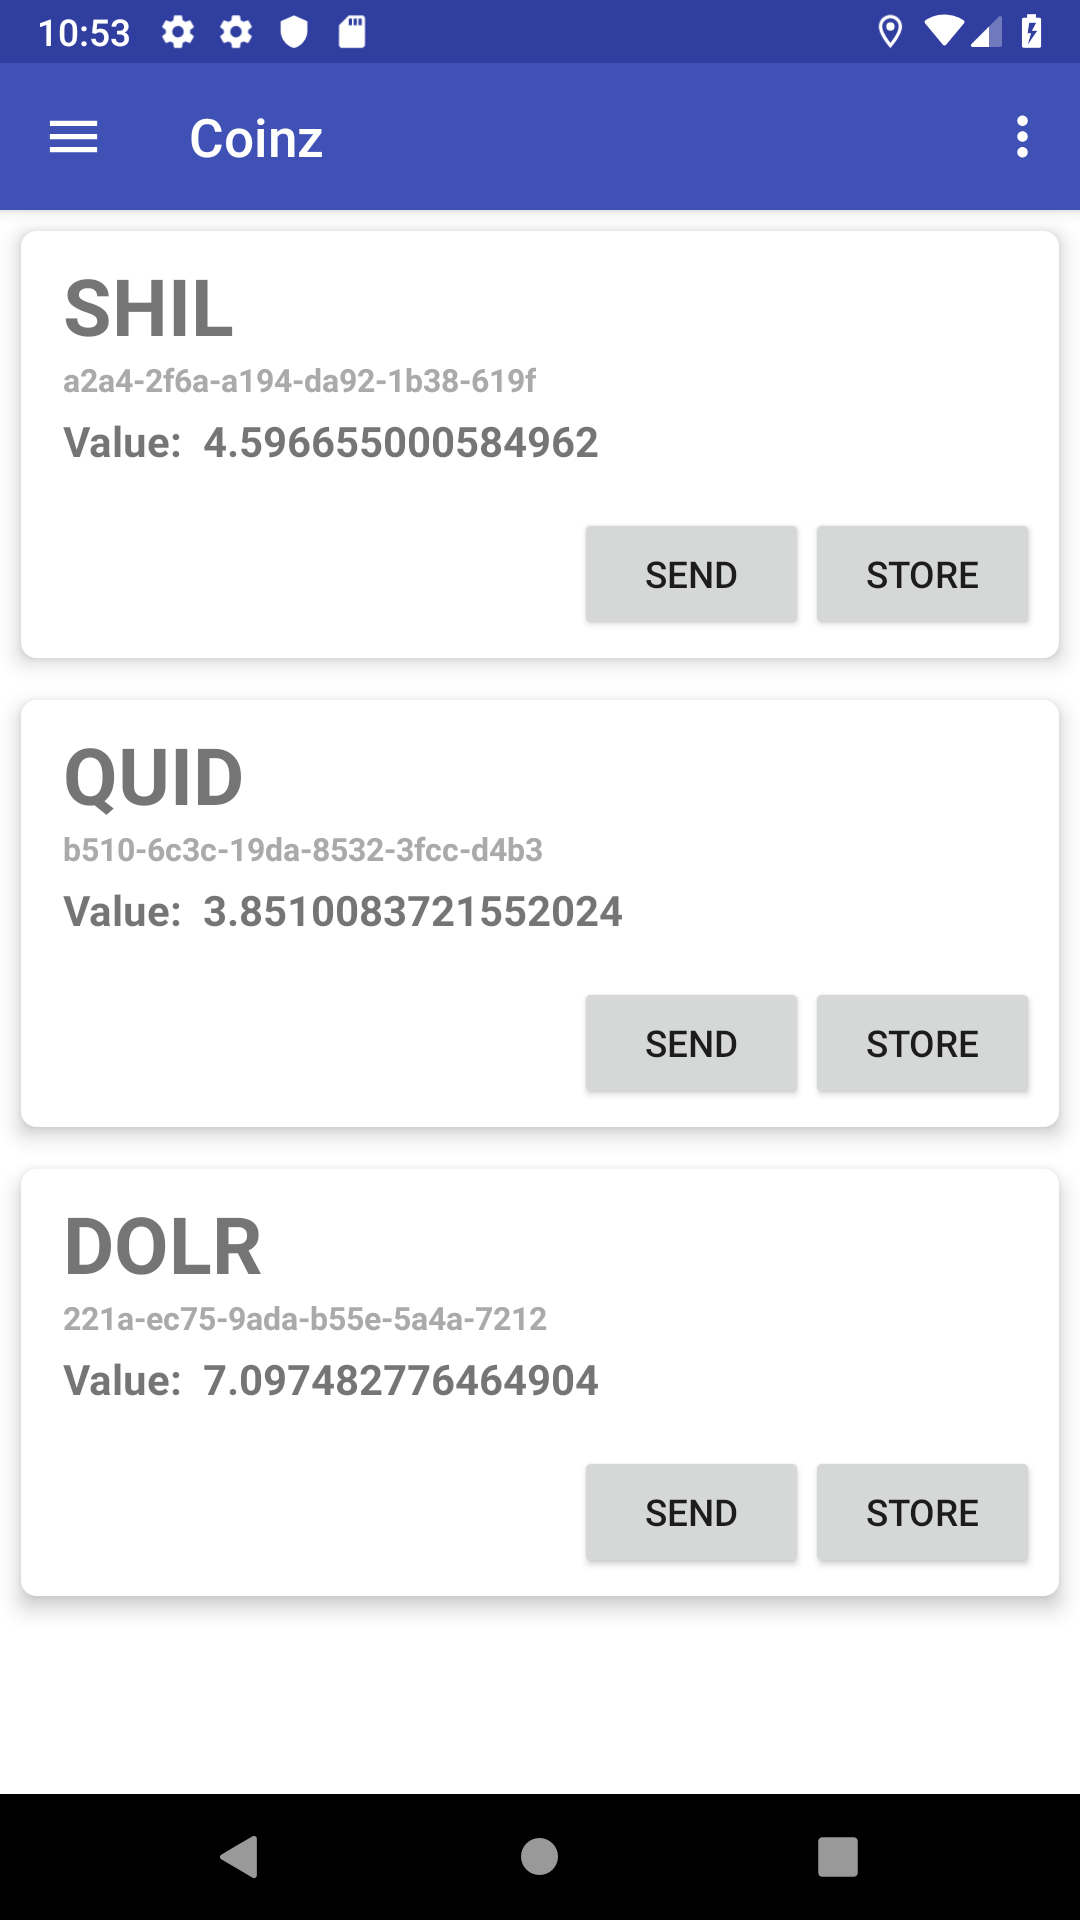
\includegraphics[scale=0.25]{screenshots/local-wallet/local-wallet-after-coin-store.png}
    \caption{Coins displayed in Local Wallet with coin ID and the stored value. Buttons to send the coin to another player or bank it into the Central Bank are also provided.}
\end{figure}

    With an increasing amount of coins in their Local Wallet the ability to display all of them on one screen will fade rather quickly. In case not all coins fit the screen, the user can simply scroll through their collected goods:

\begin{figure}[H]
    \centering
    \begin{minipage}[t]{0.48\textwidth}
        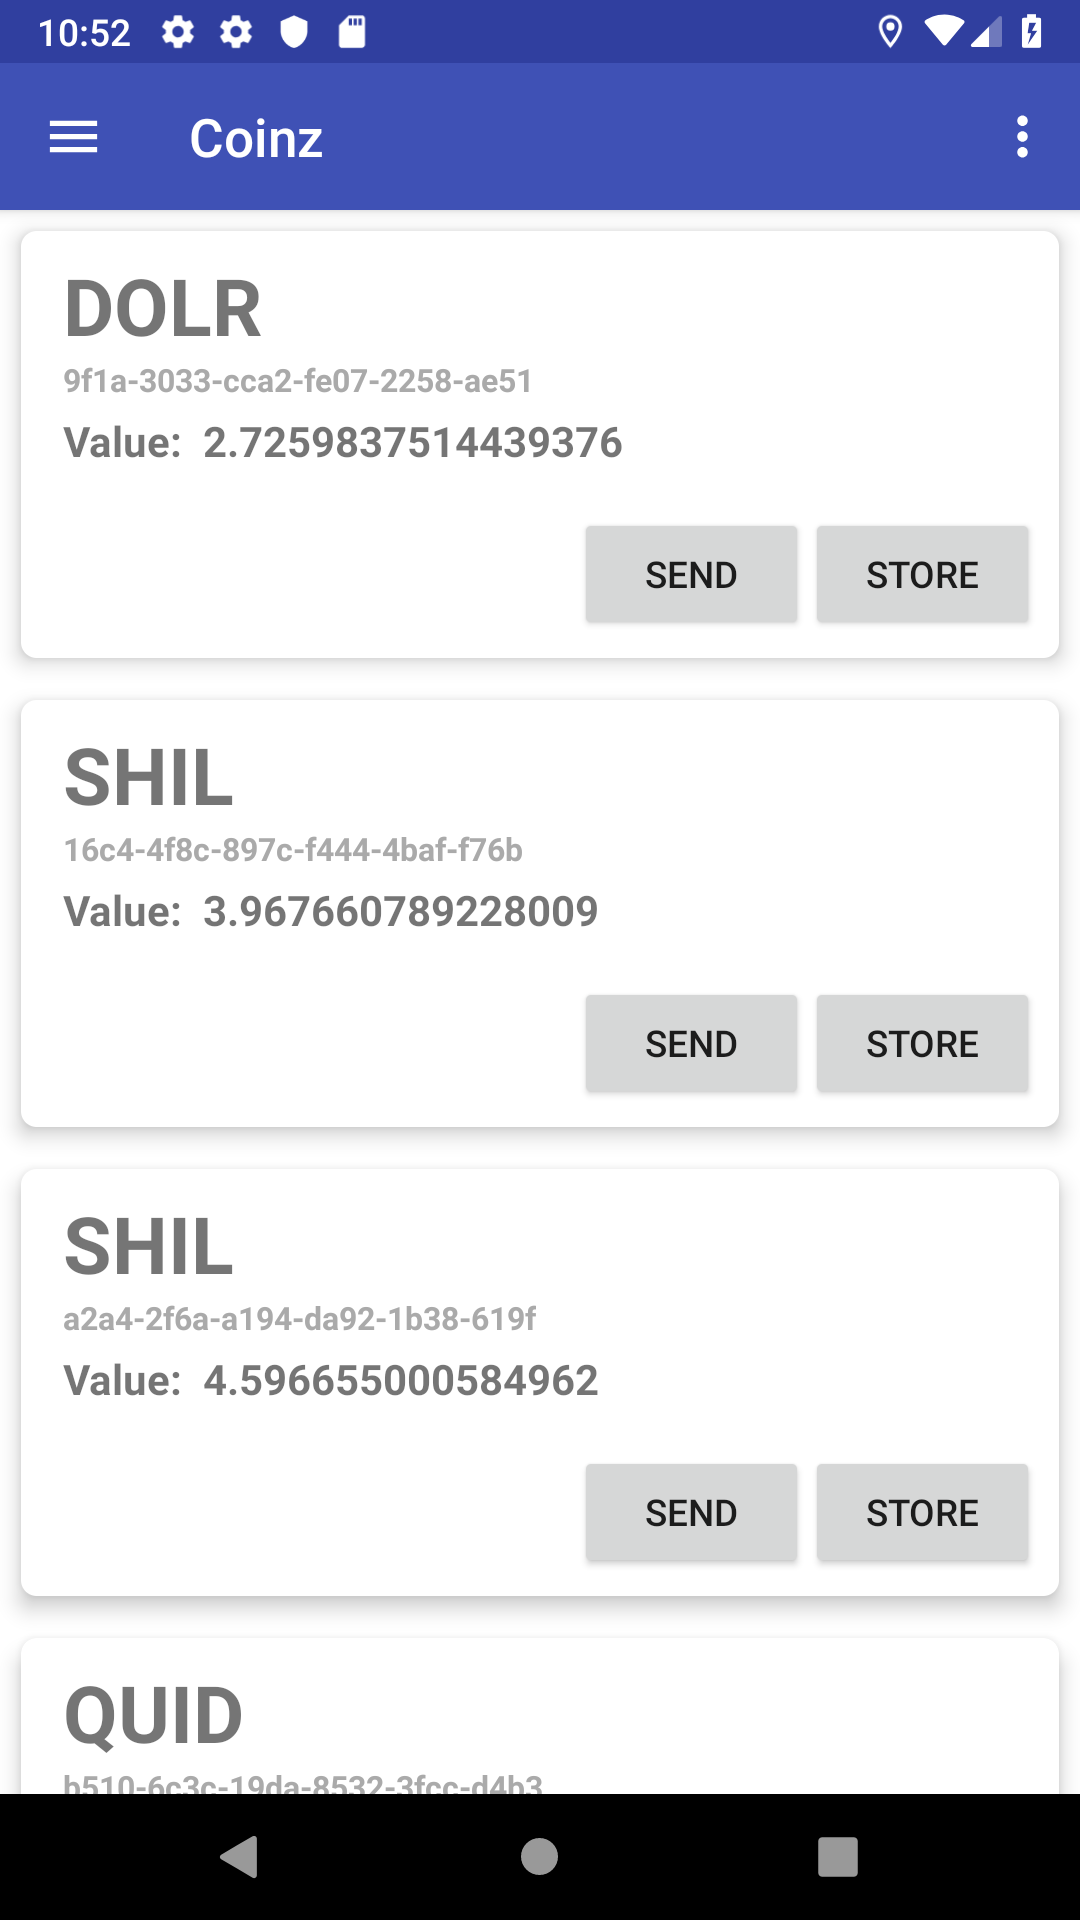
\includegraphics[scale=0.2]{screenshots/local-wallet/too-many-coins-for-screen.png}
        \caption{Opened Local Wallet with too many coins to display on one screen.}
    \end{minipage}
    \begin{minipage}[t]{0.48\textwidth}
        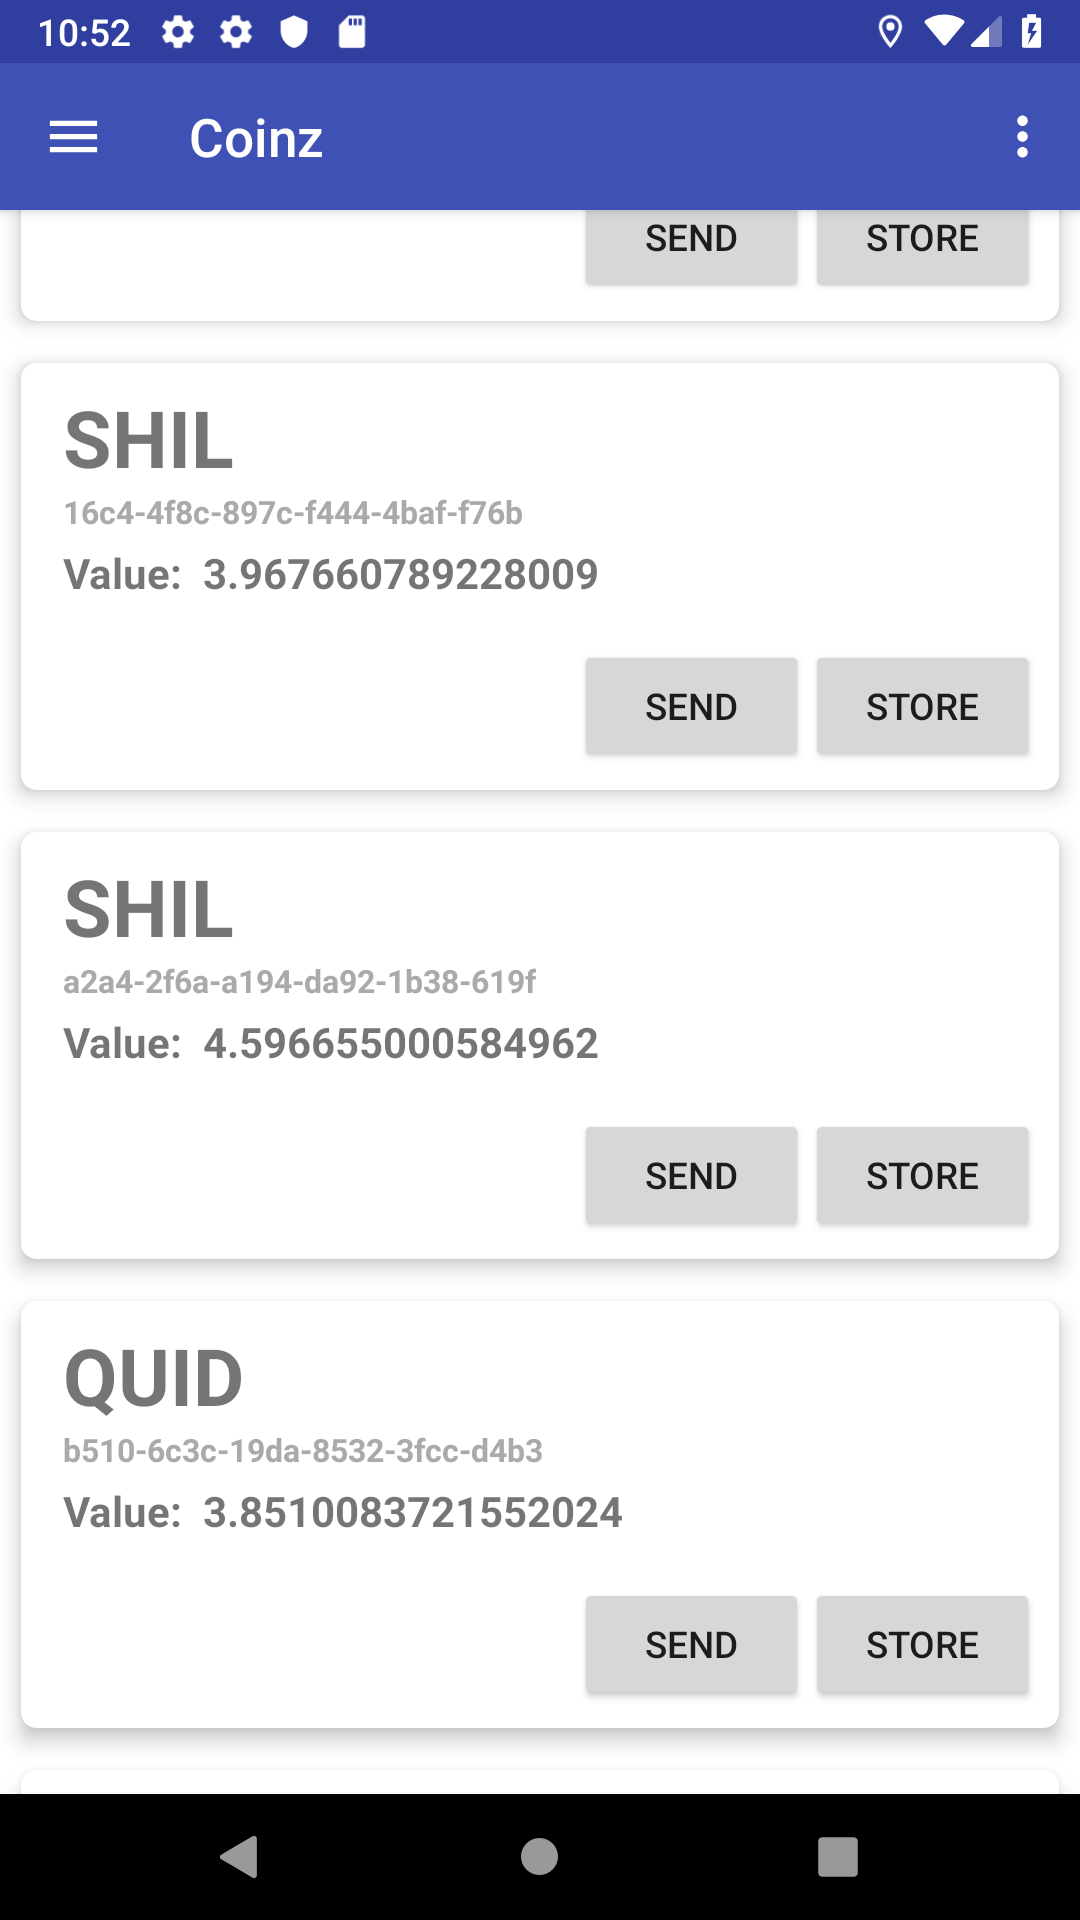
\includegraphics[scale=0.2]{screenshots/local-wallet/scrolled-down-on-coins.png}
        \caption{Scrolled down on the same list of coins to view more.}
    \end{minipage}
\end{figure}

    After having admired their progress, the user can choose to send a coin off to the Central Bank for safe-keeping by pressing the "Store" button for the particular coin the user would like to send off:

\begin{figure}[H]
    \centering
    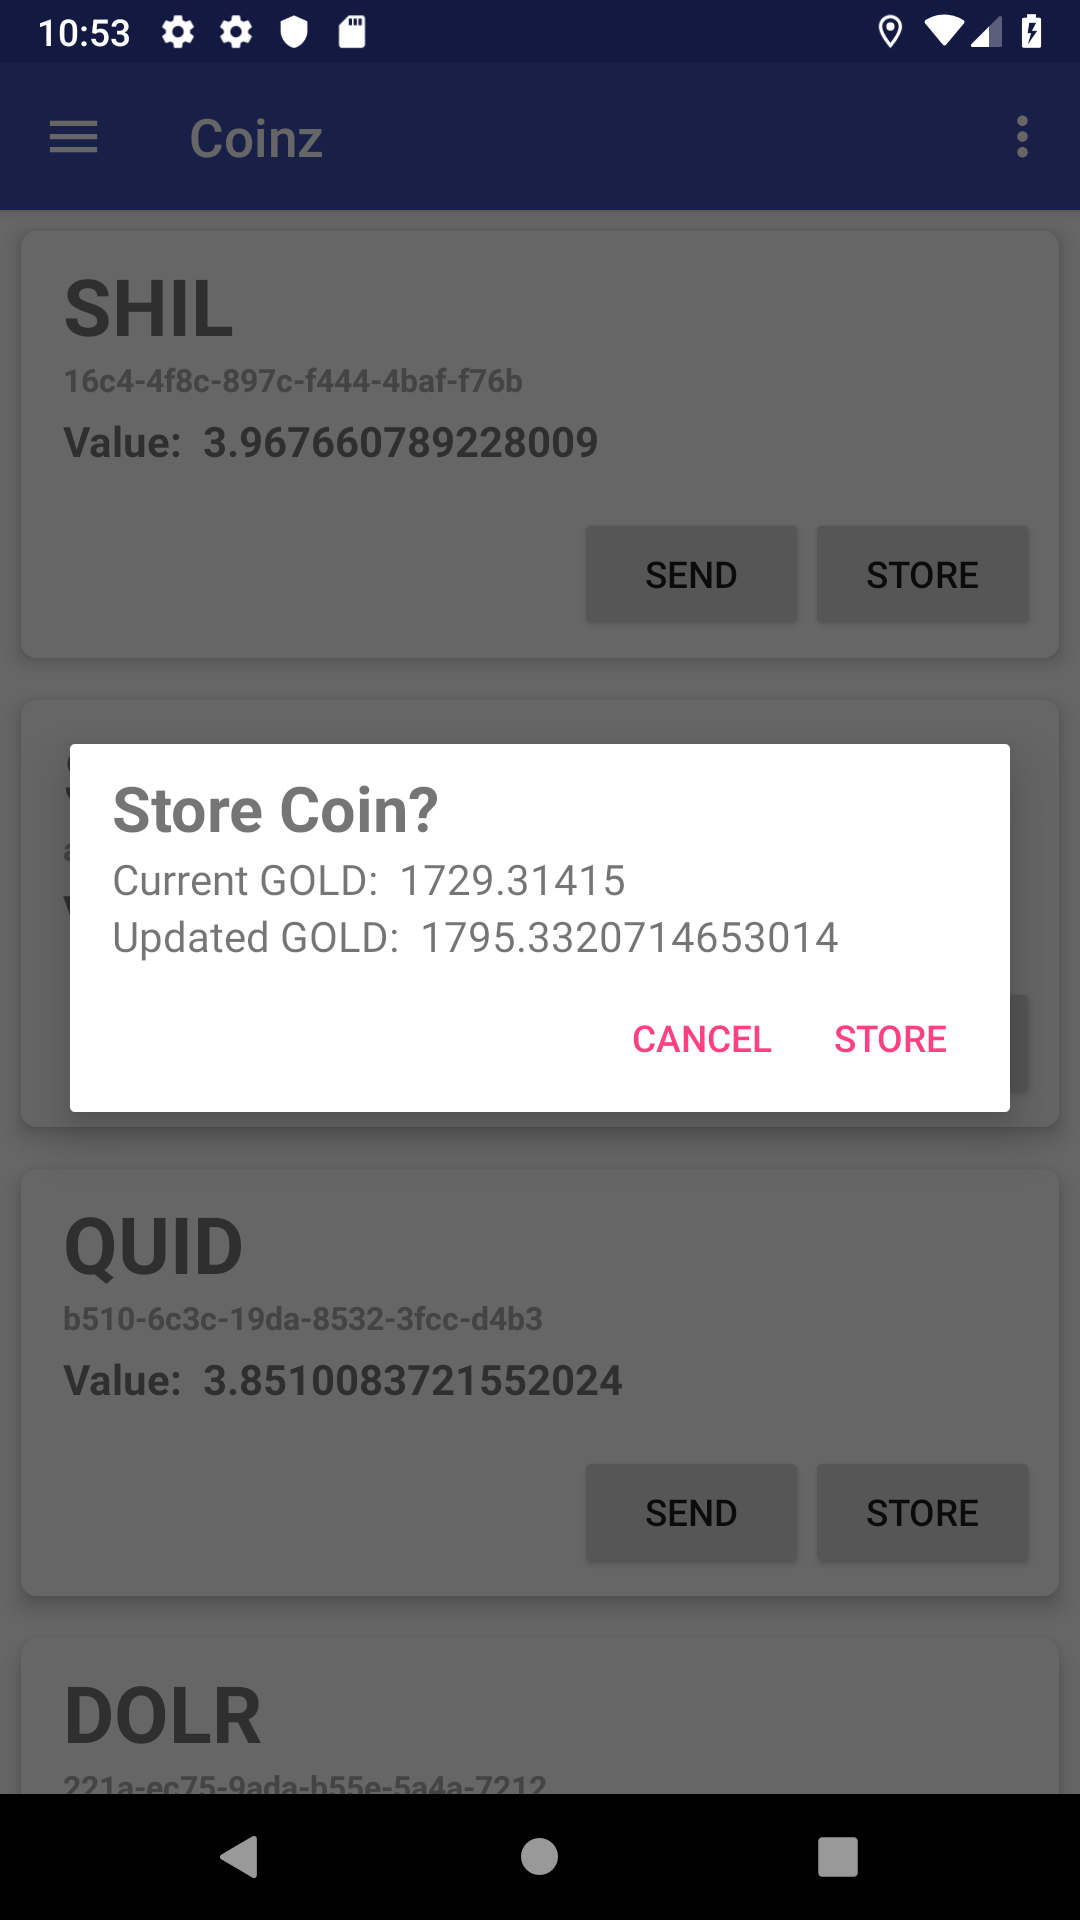
\includegraphics[scale=0.25]{screenshots/local-wallet/store-coin-dialog.png}
    \caption{Coin storing dialog showing the impact of storing that particular coin in the Central Bank, i.e. how much the coin exchanged for GOLD will increase their overall GOLD.}
\end{figure}

    Since the all coins in the Local Wallet will disappear once the date changes and a new map full of coins is downloaded, the user is advised to make use of the 25 coins they can bank each day. Once the "Store" button is pressed and given that the user can still store coins for the day, the coin will disappear from the Local Wallet:

\begin{figure}[H]
    \centering
    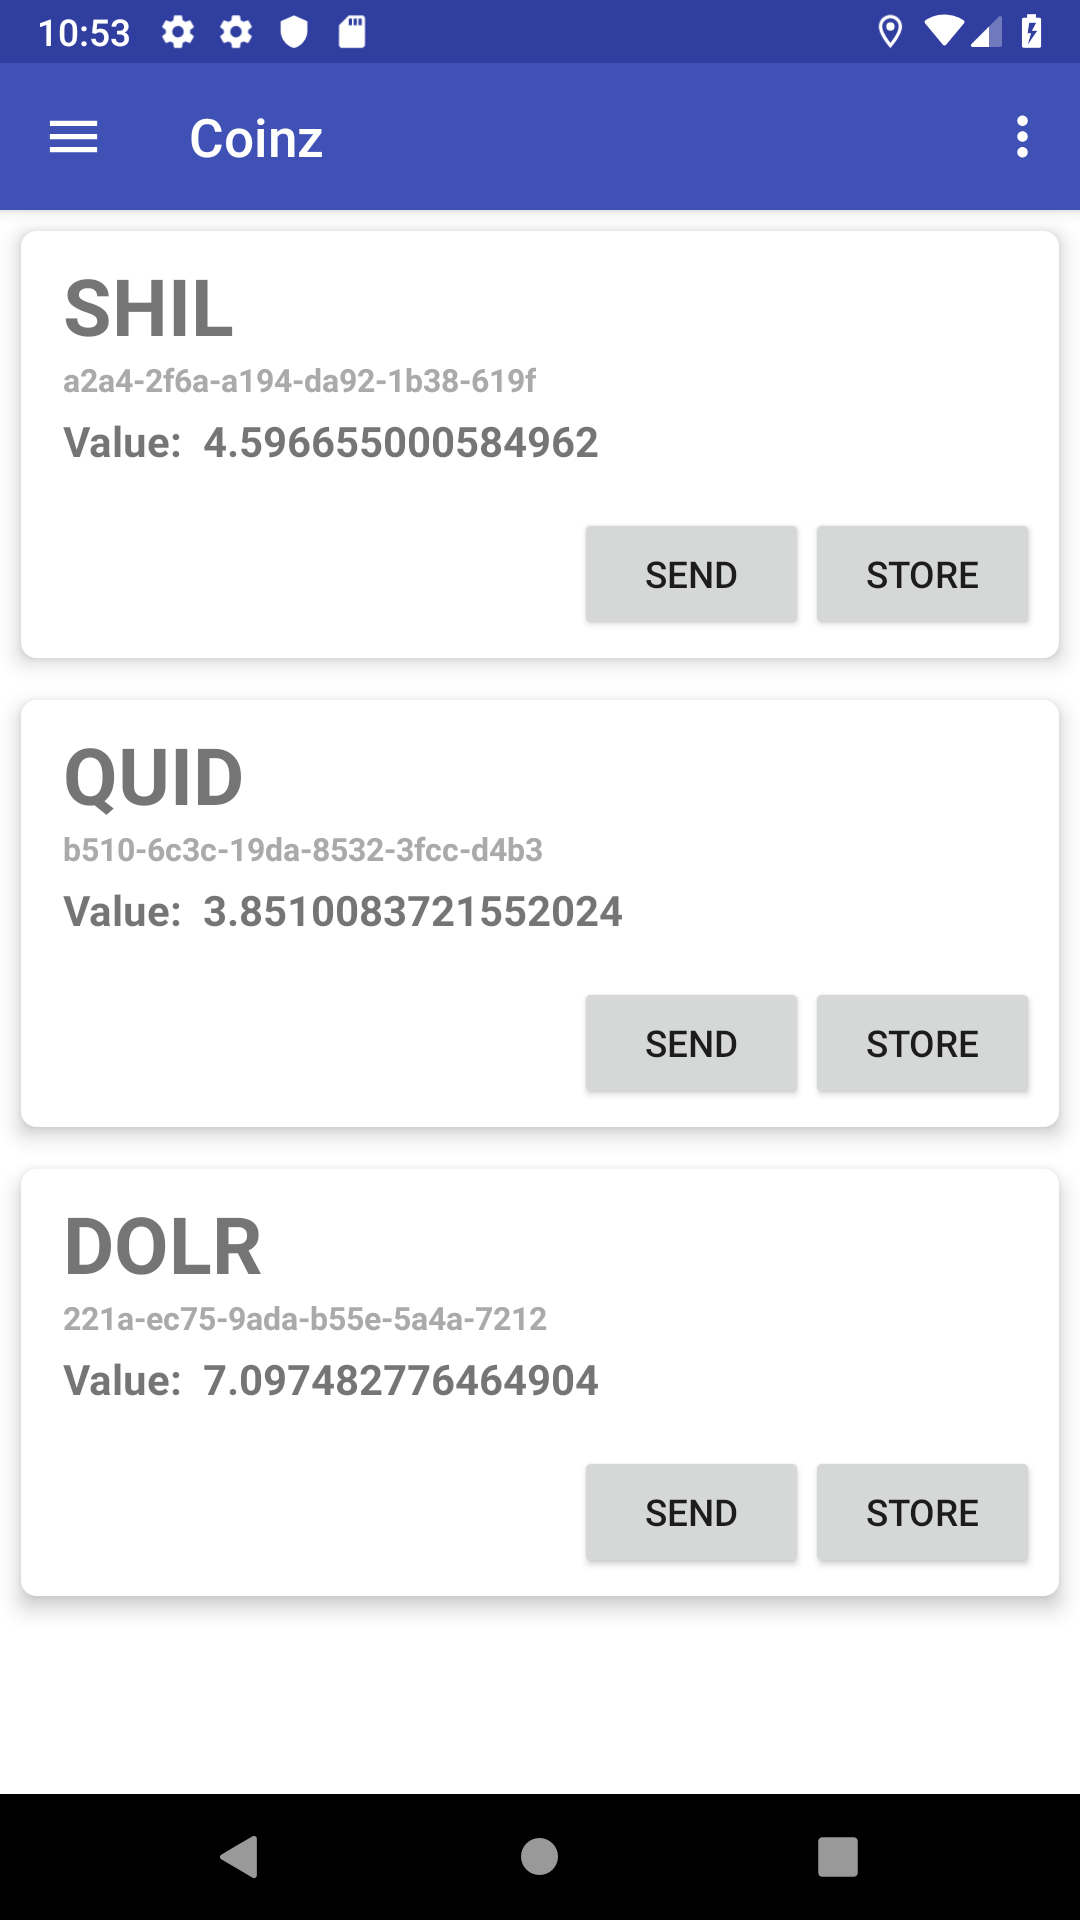
\includegraphics[scale=0.25]{screenshots/local-wallet/local-wallet-after-coin-store.png}
    \caption{Updated Local Wallet after coin has been banked.}
\end{figure}

    Now that we have seen how to bank coins it would be interesting to see what the overall GOLD amount accumulated by the user playing the game is. We therefore turn to the Central Bank.

\subsection{GOLD Rush - The Central Bank}

    In the current iteration of Coinz, the Central Bank is just a simple display of how much GOLD is stored in the user's Central Bank:

\begin{figure}[H]
    \centering
    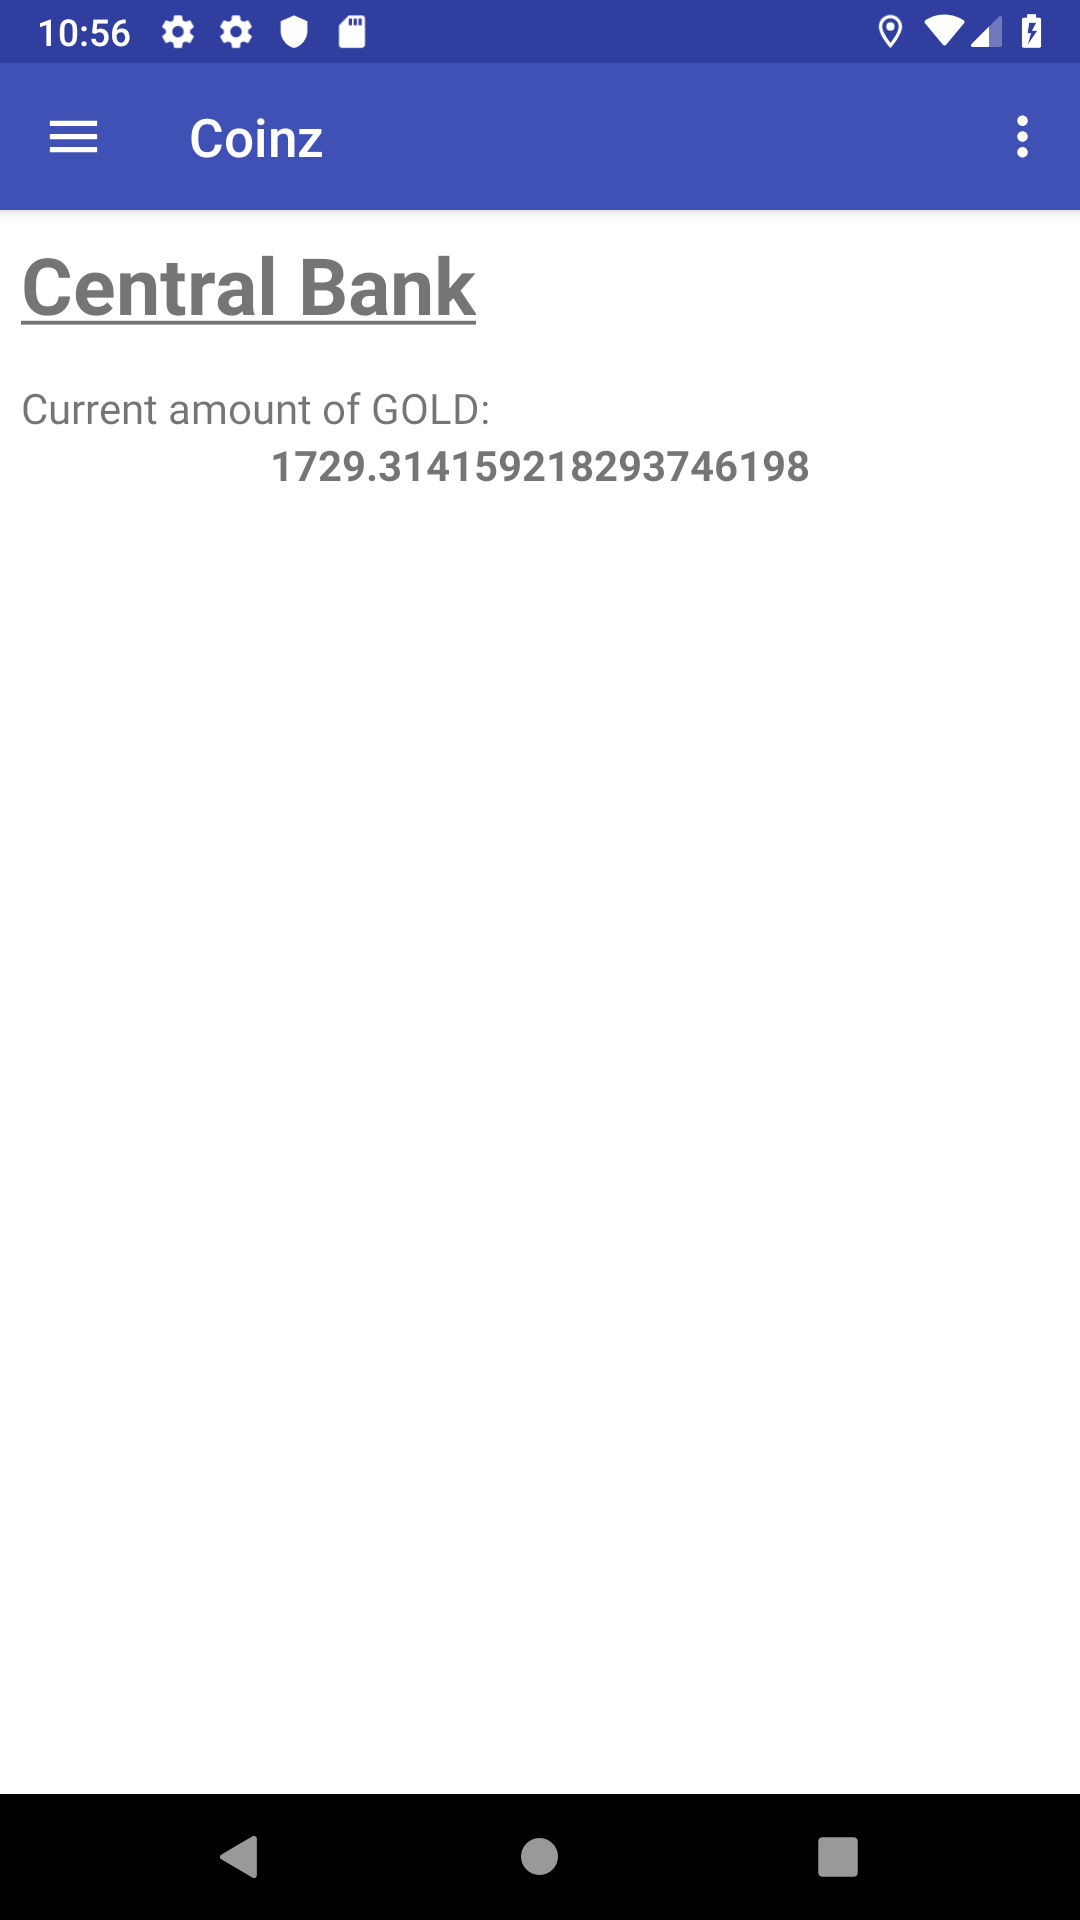
\includegraphics[scale=0.25]{screenshots/central-bank/central-bank-view.png}
    \caption{Central Bank interface displaying user's GOLD amount. Currently non-functional, so a dummy GOLD value has been put in place.}
\end{figure}

    The Central Bank, as seen above, can be accessed through the navigation drawer, just like the Local Wallet and the map.

    Hopefully the day will never come, but once the user has decided that they have played enough Coinz for now, they have the option to log out through the navigation drawer.

\subsection{Time to Say Goodbye - Logging Out (and In again)}

    To log out, all the user has to do is open the navigation drawer again and click the menu item "Log Out". They will then be taken back to the login screen and notified of their successful log out through a Toast message:

\begin{figure}[H]
    \centering
    \begin{minipage}[t]{0.48\textwidth}
        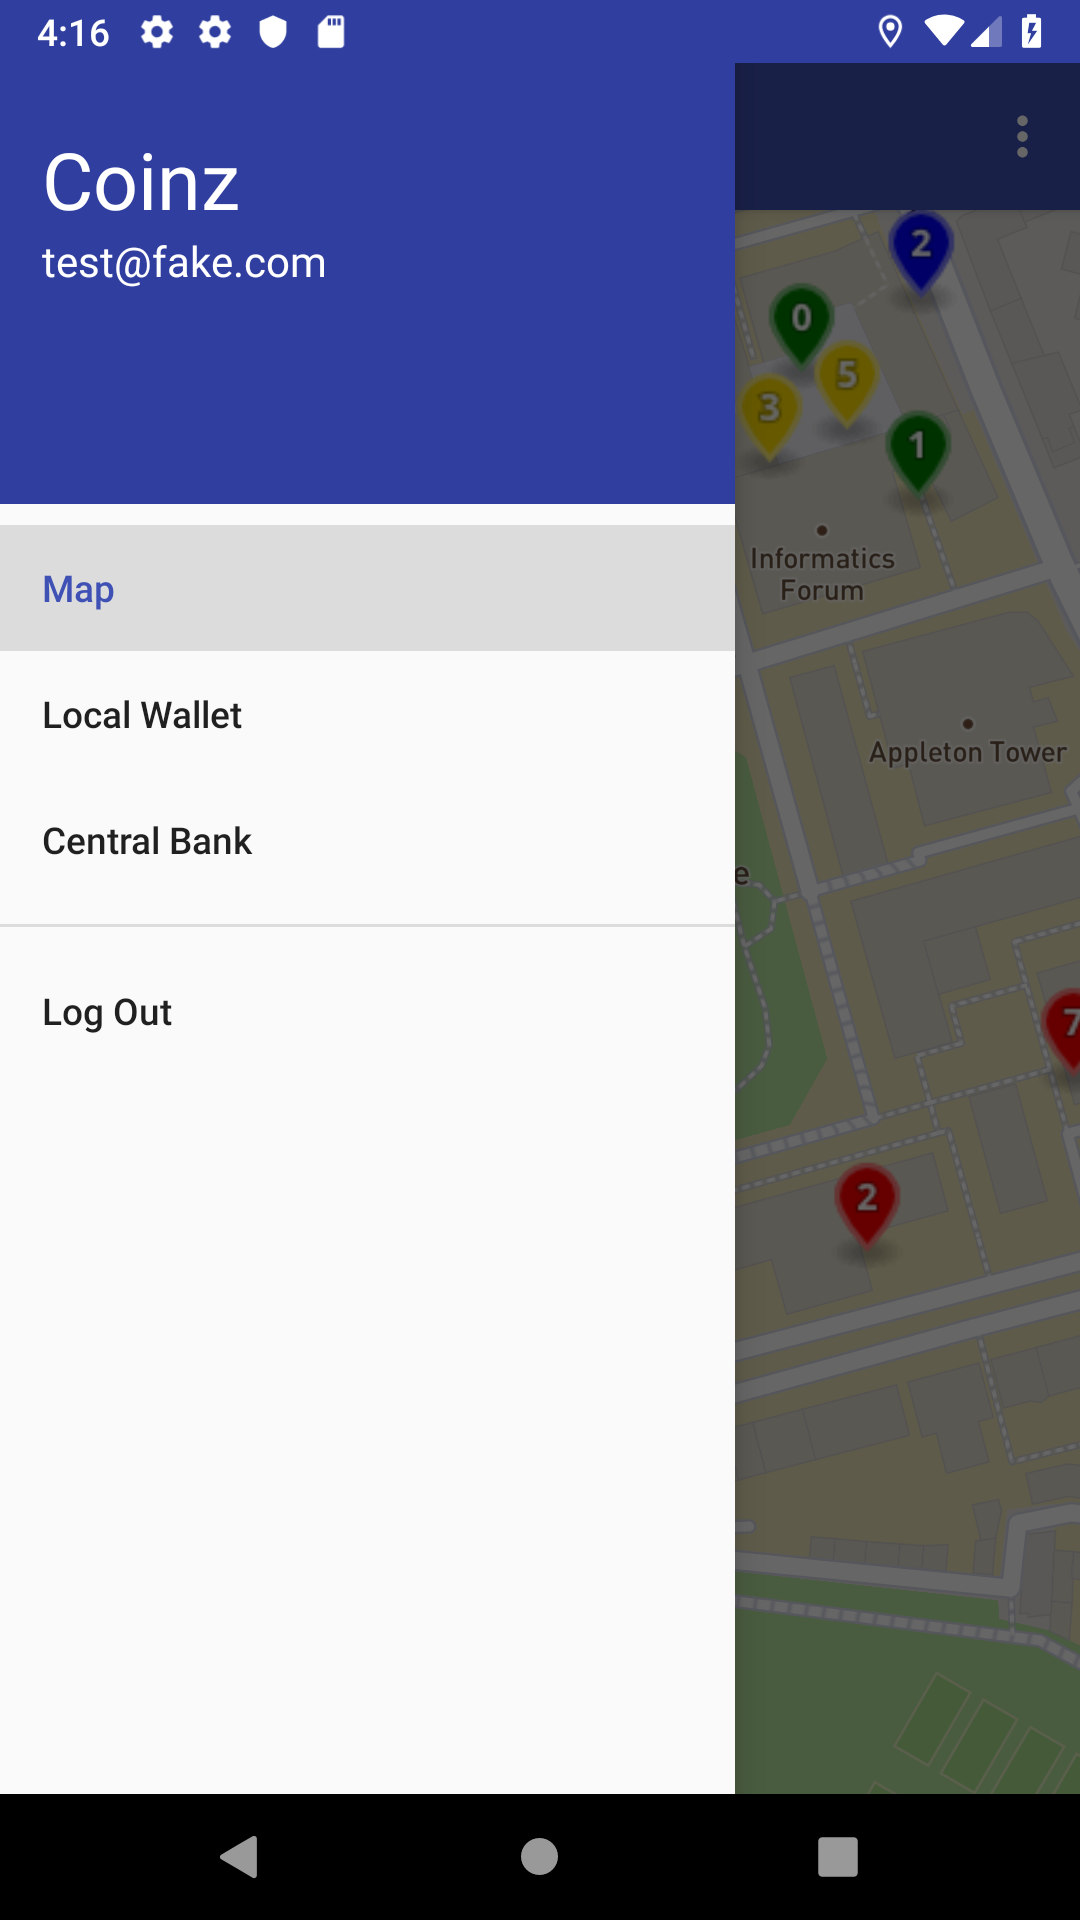
\includegraphics[scale=0.2]{screenshots/navigation-drawer/navigation-drawer-map-selected.png}
        \caption{Navigation drawer with log out menu item to log out of current Coinz account.}
    \end{minipage}
    \begin{minipage}[t]{0.48\textwidth}
        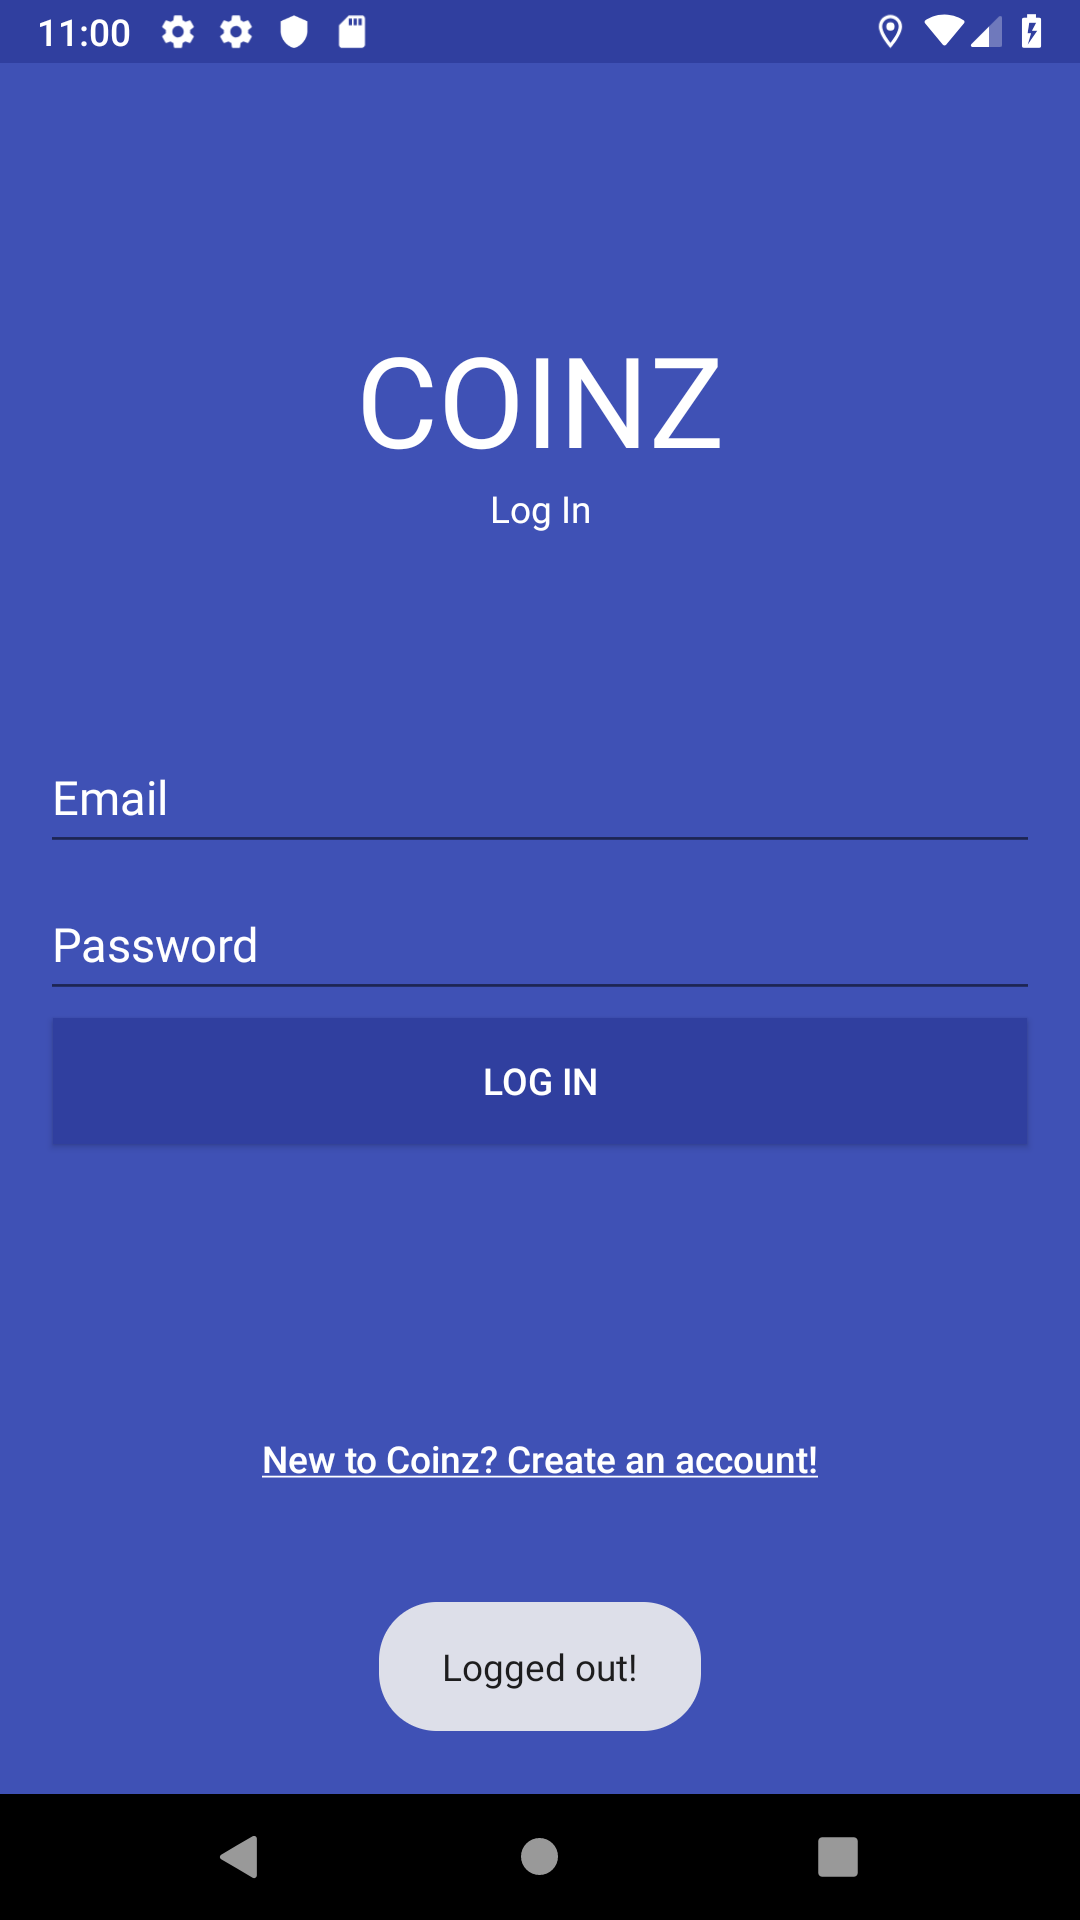
\includegraphics[scale=0.2]{screenshots/log-out/logging-out.png}
        \caption{Log in screen upon successfully logging out.}
    \end{minipage}
\end{figure}

    As the user will certainly want to continue playing Coinz at some point, they will want to log back into their account:
 
\begin{figure}[H]
    \centering
    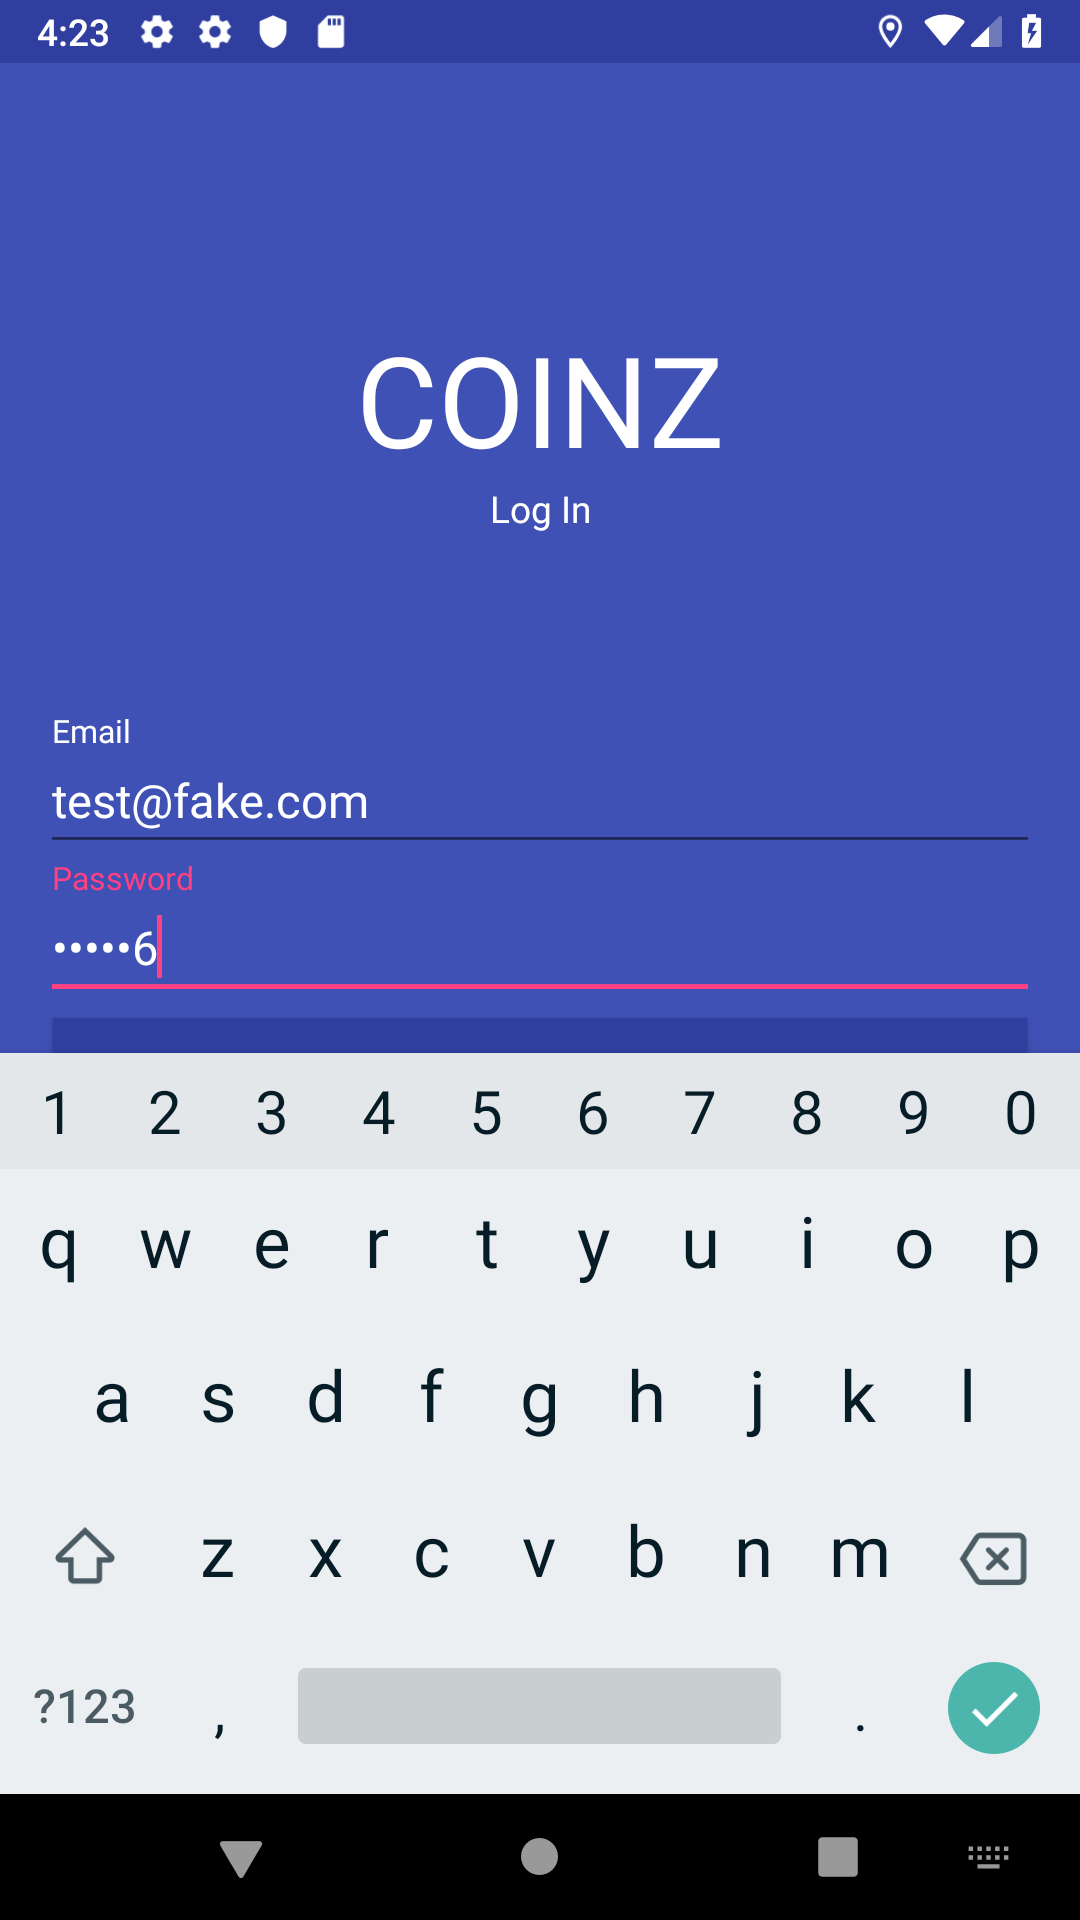
\includegraphics[scale=0.25]{screenshots/log-in/log-in-screen-logging-in.png}
    \caption{User providing the email and password linked to their account to log into Coinz again.}
\end{figure}

    Just as with the account creation, the user will be notified of the outcome of their attempt to log in:

\begin{figure}[H]
    \centering
    \begin{minipage}[t]{0.48\textwidth}
        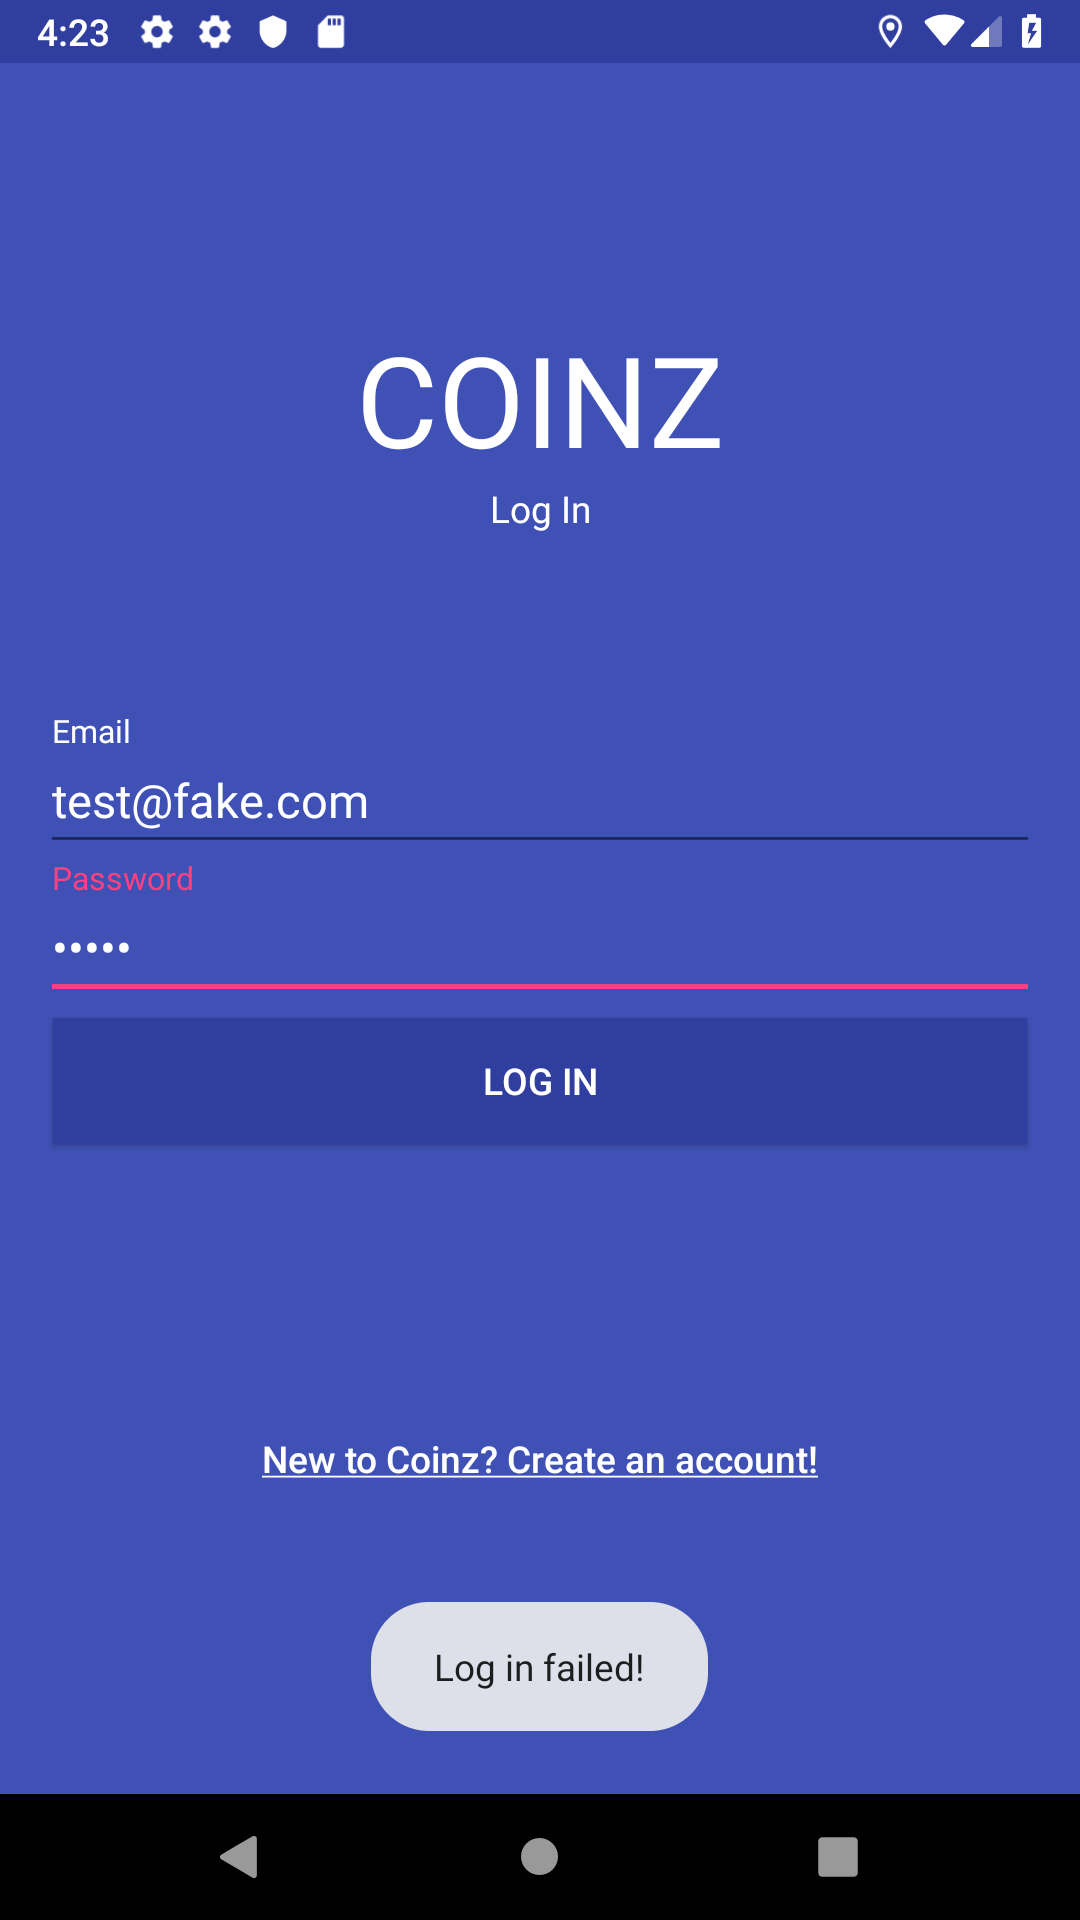
\includegraphics[scale=0.2]{screenshots/log-in/log-in-failed.png}
        \caption{Log in attempt failed}
    \end{minipage}
    \begin{minipage}[t]{0.48\textwidth}
        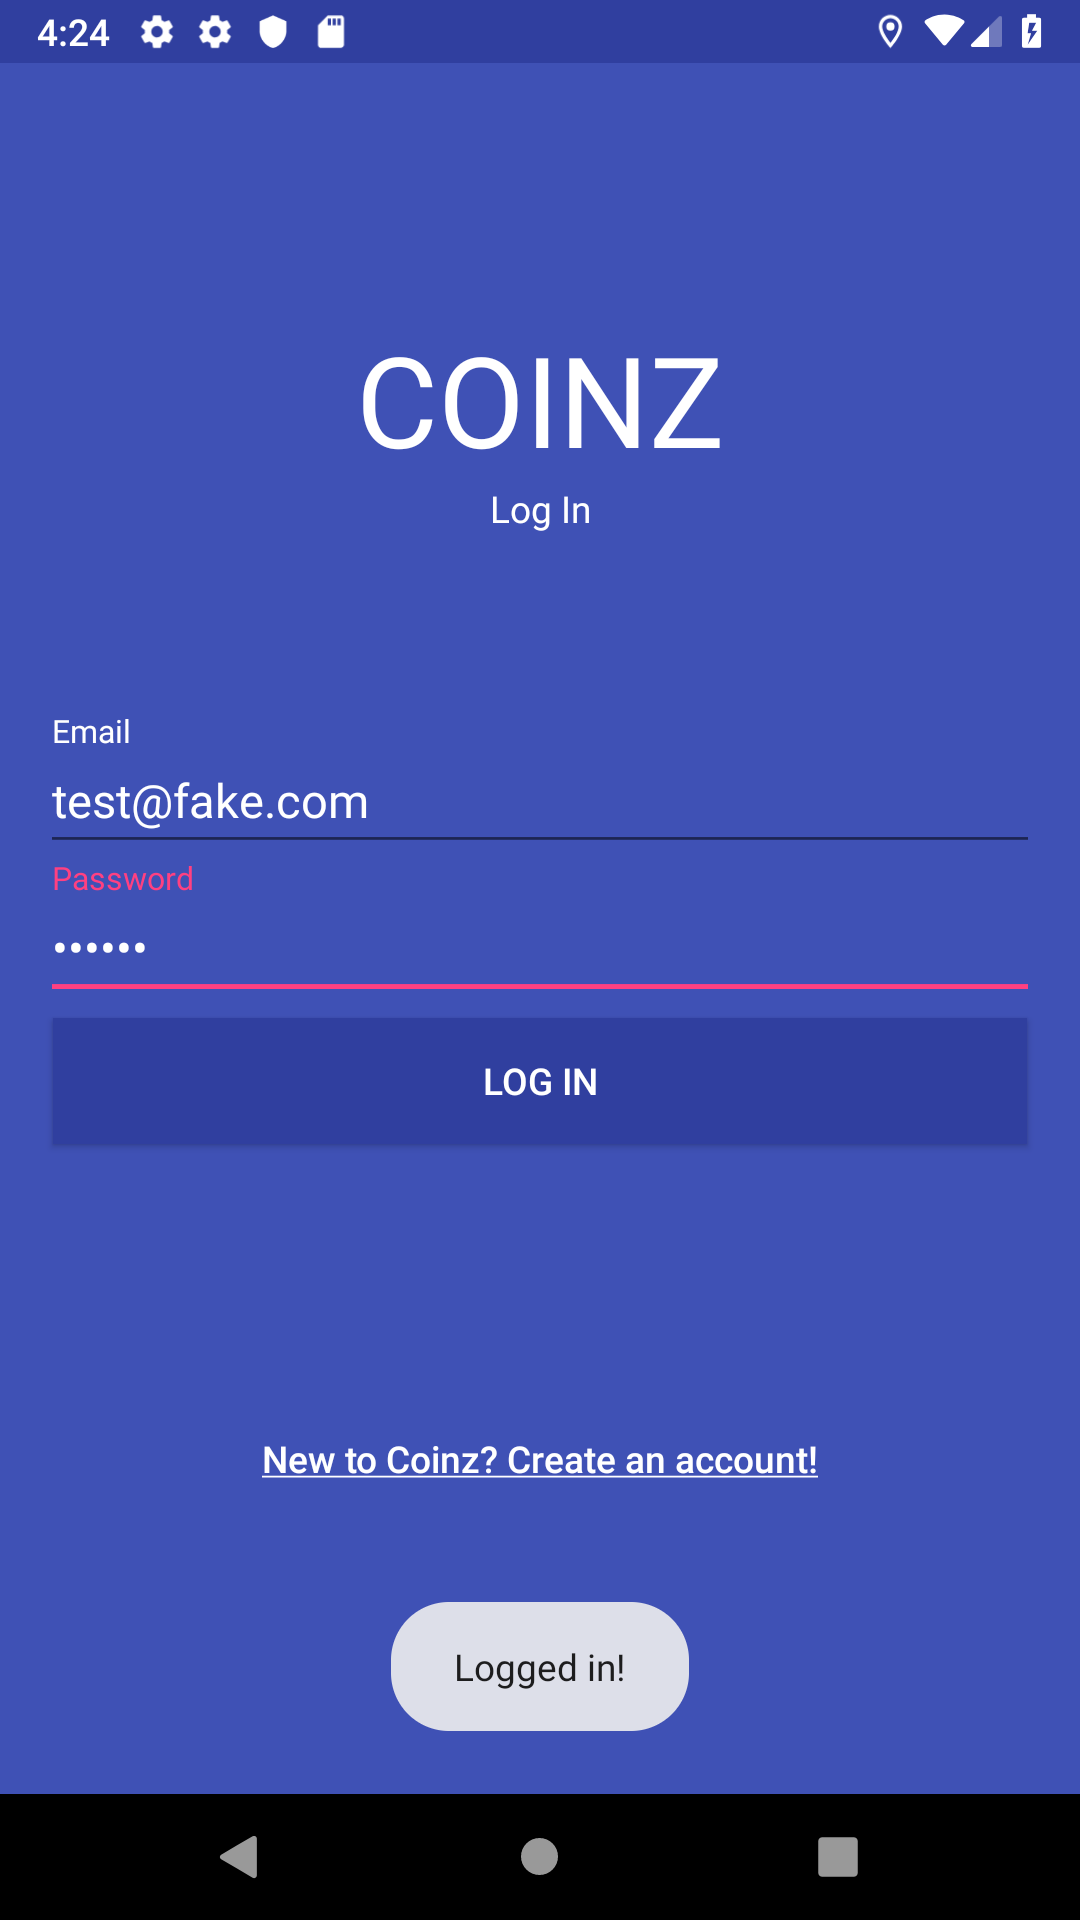
\includegraphics[scale=0.2]{screenshots/log-in/log-in-succeeded.png}
        \caption{Log in attempt succeeded.}
    \end{minipage}
\end{figure}

    In the case that the login is successful, just like after the account creation, the user will be moved over to the Coinz map to start playing some more. Another similarity to the account creation is that in the current version of Coinz, the reason why the login attempt did not succeed will not be displayed to the user. It could be, for instance, that their password is incorrect.

    This concludes a typical run through the Coinz app from creating an account, to playing on the map to logging back out of the account and it therefore also concludes the application showcase.

\section{Acknowledgments}

    \begin{itemize}
        \item \emph{Room Database}. The entirety of the persistent local storage code using the Room Persistence Library is adapted from the "Android Room with a View - Kotlin" codelab. \cite{room-tutorial}

        \item \emph{Dialog Fragments}. Each fragment inheriting from the DialogFragment class includes code that is adapted from the official Android developer site. \cite{dialog-tutorial}

        \item \emph{Navigation Drawer}. The implementation of the navigation drawer is, for the most part, taken from the official Android developers tutorial page, with adaptions where needed. \cite{nav-drawer}

        \item \emph{Login and Account Creation}. The implementation of the login and account creation screens are mostly adapted from AndroidHive. \cite{firebase-login}

        \item \emph{Cloud Firestore}. Any code related to Firestore is adapted from guides found on the official Cloud Firestore guides site. \cite{firestore-guides}
    \end{itemize}

\section*{Special Thanks}

    \textbf{\emph{Dr. Stephen Gilmore}}. I would like to sincerely thank him for a wonderful introduction into Android programming. It was truly a pleasure to attend his lectures and the fact that he does not get to see this course through to the end and see all of the wonderful applications built under his lead is nothing but heartbreaking to me. I wish him all the best and hope I will get to have him as a professor again.

    %\emph{Pavlos Andreadis}. While we were ultimately unable to resolve the issue that caused my application to seemingly crash at random, he was still able to help me narrow the issue down to Firestore related code and gave me some guidance on how to somewhat save my final submission.

\newpage
\printbibliography

\end{document}
